%!TEX root = ../physical-olympics-2.tex
\chapter{导体与介质}




\section{导体与静电平衡}

\subsection{绝缘体与导体}



微观地看,\,物质由原子或分子等组成,\,其中导电现象通常发生在不同情况下:

	\vspace{0.3cm}1. 真空导电:\,一般不会说真空具有\emph{导电性}(conductive),\,因为真空中是没有\emph{载流子}(charge carrier)的\footnote{量子场论认为真空存在电子对的产生湮灭涨落从而具有一定的导电性.}.\,的确,\,在\emph{阴极射线管}(cathode ray tube)中,\,加热一个阴极,\,并辅以合适的偏置电压可以造成真空中的电流.\,或是用一束能量足够的光子去轰击金属表面造成电子逸出,\,甚至纯粹由于阴极表面尖处十分强的电场导致电子直接克服逸出功发射出来.\,三种现象分别称为\emph{热发射}(thermionic emission),\,\emph{光电效应}(photoelectric effect)与\emph{场发射}(field emission).这种电荷的定向移动现象被统一地称为\emph{输运现象}(transport phenomenon).\,由于真空输运的独特性质,\,比如电子不会受到散射,\,平均自由程远大于仪器尺寸,\,与凝聚态物理中的一些概念对应,\,这被称为\emph{弹道输运}(ballistic transport).

	\begin{wrapfigure}[16]{o}[0pt]{5cm}
	\vspace{-1.6cm}
	\centering
	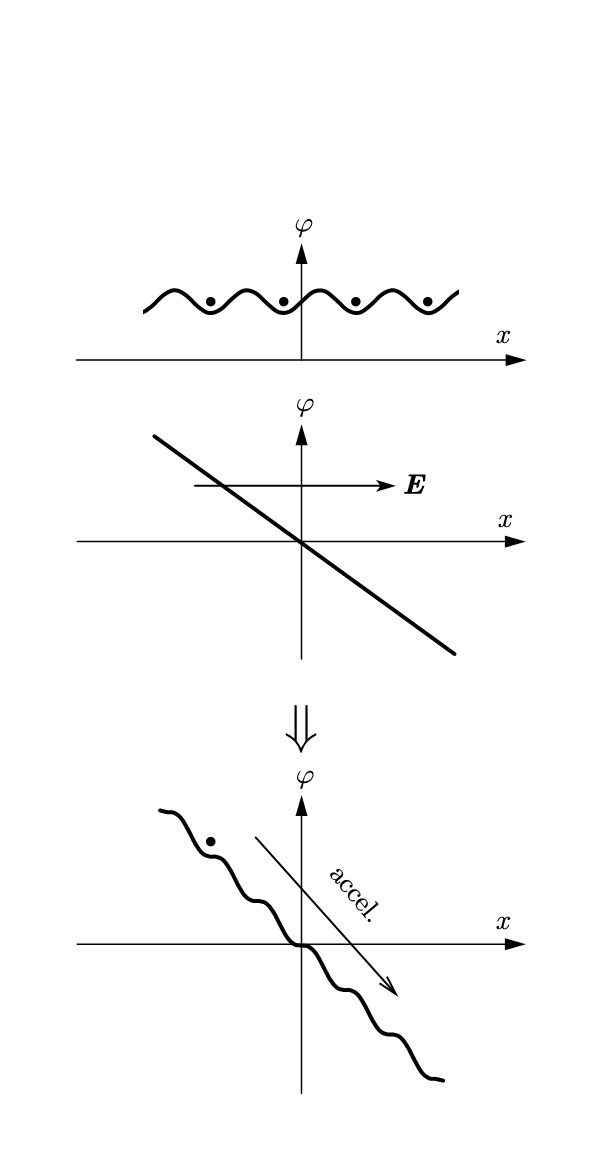
\includegraphics[width=5cm]{image/7-2-1.png}
	\caption{晶体击穿}
	\end{wrapfigure}

	\vspace{0.3cm}2. 绝缘体漏电:\,大多数非金属晶体,\,或是不含离子的液体与气体,\,原子核在晶体中都限制在点阵格子的特定位置,\,在气体,\,液体中则是可以活动的原子分子周围.\,电子分为两类,\,,一类是原子的内层电子,\,它极为稳定地存在于原子周围,\,离子晶体中的几乎完全被阴离子夺取的电子也属于这种情况.\,它们与原子核一起构成\emph{原子实}(atomic core).\,而\emph{价层电子}(valence shell electron),\,它们用来成键,\,将原子连接形成分子或者晶体,\,一般被定域在原子间的特定区域.\,所有这些电子的特点都是\emph{束缚态}(bond state).\,它们不能在介质中自由传导,\,一个电子的区域到另一个电子的区域间存在\emph{势垒}(potential barrirer),\,经典物理认为电子的动能不足以穿过这些势垒.\,但是,\,量子理论则认为电子的波函数可以通过\emph{隧道效应}(tunnelling)以小概率在不同区域间转移.\,这就为有电场的情况下电荷的平均定向移动提供了可能.\,这种现象称为\emph{漏电}(leakage).

	\vspace{0.3cm} 3. 绝缘体击穿:\,在十分高的电场下,\,原子与原子间,\,或是分子中显不同电性的部分之间的典型电压将大于阻碍电子转移的势垒.\,在晶体被击穿时此时电子在本质上可以被视为在周期性势能场与线性势能场的叠加中运动的经典粒子.\,不难看出电子不仅可以脱离单个势阱的束缚,\,还可以在这样的电场力下做持续的加速运动.\,气体液体则是在电场力作用下原子,\,分子被撕裂为离子而继续在电场力下做加速运动.\,此时碰撞就发生了:\,碰撞的结果往往是使得更多的原子分子发生电离.\,这样就会雪崩式的累积,\,固液气中的这些现象都称作\emph{雪崩击穿}(avalanche breakdown).\,尤其是气体中的放电现象在不同电流条件下分别造成\emph{汤森放电}(Townsend discharge),\,\emph{电晕放电}(corona discharge),\,\emph{辉光放电}(glow discharge),\,\emph{电弧放电}(arc discharge)的不同情况.

	\vspace{0.3cm} 4. 自然的导体:\,我们将材料区分为\emph{绝缘体}(insulator)与\emph{导体}(conductor),\,最重要的依据就是在弱场下是否天然地具有能产生电荷输运的载流子.\,所以导体就是一类事先就具有一定数密度$n$的一种或多种载流子$q$的材料,\,它们往往在有电场$\bs{E}$在场时发生位移,\,且与散射造成的形式阻力平衡,\,造成平均的匀速运动,\,即\emph{定向漂移}(directional drift).\,常见的金属以最外层的自由电子为载流子,\,半导体以热激发或掺杂形成的电子或空穴为载流子,\,电解质溶液或部分气态或液态的等离子体以阴阳离子为载流子.\,它们都是典型的导体.\,区别于前三种情况与最后的超导体.

	\vspace{0.3cm} 5. 超导体:\,低温下的很多奇异的宏观现象大大拓宽了人们对量子理论在物理学各个层次中应用的认识.\,其中很典型的一个就是\emph{超导}(superconductivity)现象.\,最早在1911年由\emph{昂内斯}({\it H. K. Onnes})在研究低温下汞的电阻率时惊人的发现在$4.2{\rm K}$下电阻率消失至零,\,这就是超导的发现.\,但是直到约十年后才引起足够重视.\,在$1933$年\emph{迈斯纳}({\it F. W. Meissner})才发现超导不仅仅是电阻率的消失,\,还伴随着\emph{完全抗磁性}(perfect diamagnetism):\,就好像理想导体内部无电场线,\,在超导体中交变的磁场也只能存在于表面极小的深度内(趋肤深度),\,也称\emph{迈斯纳效应}(Meissner effect).\,后来通过量子理论的蓬勃发展,\,在$1957$年提出的\emph{BCS理论}(Bardeen-Cooper-Schrieffer theory)终于解释了超导的成因,\,原来是一对\emph{库珀电子对}(Cooper pair)通过与声子(晶格振动)相互作用而造成了没有任何散射的量子模式.\,完整地解释了直到1986年所有\emph{低温超导}(low-temperatre superconductivity)的现象.\,但是随着$35{\rm K}$超导的镧钡铜氧体的发现,\,宣告人类进入\emph{高温超导}(high-temperatre superconductivity)纪元.\,新的超导材料不断被发现,\,新的理论也不断被提出,\,目前最``高温''的材料是汞钡钙铜氧体,\,超导临界温度$135{\rm K}$.\,为什么有高温超导?\,高温超导的临界温度如何进一步提高?\,直到今天这也还是方兴未艾的研究领域.\,其在科研,\,科技,\,生产,\,生活方面的应用是不可估量的.

\vspace{0.5cm}

我们将把研究的范围主要放在导电的导体和不导电的绝缘体上.\,前者分析其静电平衡,\,即本章要集中讲的情形;\,下一章的稳恒电流和之后章节的拟稳的一些情况则是导体研究的其他场合.\,对于绝缘体我们本章也介绍其介电特性,\,光作为电磁波在介质中的传播则本章做一个抛砖引玉,\,主要内容在光学色散理论中讲解.

\subsection{导体的特点}

这里说的导体,\,主要指固体形式的金属.

首先界定我们研究的问题范围:\,\emph{静电平衡}(electrostatic equilibrium)问题是一种\emph{稳态}(steady state).\,我们研究的问题由各式各样的,\,有限的块状导体${\rm C}_1,\,{\rm C}_2\cdots {\rm C}_n$构成,\,这些导体带电情况由体电荷密度$\rho$和面电荷密度$\sigma$描述.\,但是导体${\rm C}_i$上的总电荷量不一定为零:
\[Q_i=\int\limits_{{\rm C}_i}\rho \ud V+\int\limits_{\partial{\rm C}_i}\sigma \ud S\neq 0\]

这个电量$Q_i$一般也是可以在一定范围内人为控制的,\,即给导体\emph{充电}(charge).\,利用电容的性质很容易可以做到这一点.\,在为导体充电后由于电量守恒,\,其总电量就不能改变了,\,但是其电荷分布一般是未知的.


除了它们往往还有人为指定的各种点电荷$q_j$或者电荷分布$\rho(\bs{r})$存在于导体外.\,那么,\,容易想像,\,当导体外突然产生电荷分布时(如原来中和的电荷被重新分开),\,或者导体被置入电荷体系中,\,本质上就是当导体外的场环境发生改变时,\,导体内部显然不可能保持电场强度始终为零.\,只要有电场就会引起电流,\,它必然使得内部和表面的电荷分布发生改变$\dot{\rho}(t),\,\dot{\sigma}(t)\neq 0$.\,这些状态就是\emph{暂态}(transient state).\,但是只要外界的场不再变动,\,经过特征的\emph{弛豫时间}(relaxation time)后,\,一般很短只有$10^{-14}{\rm s}$量级,\,就会接近,\,直到变成稳态.

通过以上推理,\,足以看出,\,\emph{静电平衡下,\,导体内部应当没有电场.}\,这就是静电平衡理论的初始命题.\,它的初步推演泛化出以下的九宫格式的结论,\,分别讨论导体内,\,导体表面,\,导体外三处的电荷分布,\,电场分布,\,和电势分布三个特性:

\begin{table}[H]
\centering
\begin{tabular}{|c||c|c|c|}
\hline
一般特征	&电荷		  		&电场&电势\\
\hline\hline
导体内 		&$\rho = 0$			&$\bs{E} = 0$	&$\varphi=C$\\
\hline
导体表面	&$\sigma\neq 0$ 	&奇异			&$\varphi=C$\\
\hline
导体外 		&$\rho \neq 0$ 	&$\bs{E} \neq 0$&$\varphi\neq C$\\
\hline
\end{tabular}
\caption{静电平衡的初级结论}
\end{table}

其实就是说,\,因为导体内部没有电场,\,所以导体内部也没有形成电场的电荷(高斯定理可证),\,也使得导体成为一个\emph{等势体}(equipotential body),\,导体表面成为一个\emph{等势面}(equipotential surface).\,注意,\,这里说的``内部'',\,``表面'',\,``外部''包含两种情况.\,导体内部就是金属成分的空间,\,外部一般是真空与外加电荷分布的空间,\,表面是它们的分界面,\,但是下图左的情况,\,导体的外部延伸到了无穷远,\,这种为\emph{开外界}(open exterior),\,但是中和右两种情况,\,导体的外部是有限的\emph{闭外界}(closed exterior).\,第二种典型情况这个单连通的闭外界还被称作\emph{空腔}(cavity).\,除非特殊说明,\,我们一般默认导体的内部不会延伸到无穷远(总是闭的).

\begin{figure}[H]
\centering
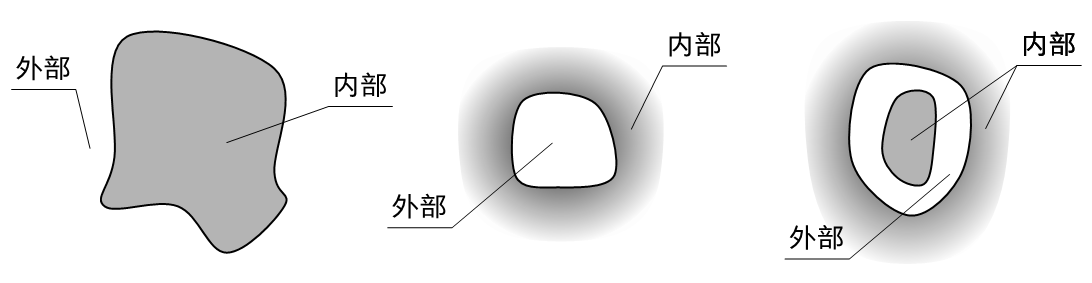
\includegraphics[width=0.7\textwidth]{image/7-2-2.png}
\caption{导体内外}
\end{figure}

在导体表面发生了电场计算的奇异性,\,因为这里是面电荷分布.\,我们考察细节就会进一步发现以下进一步的结论:\,\emph{导体表面的面电荷只朝外侧发出(或吸收)电场线,\,其方向垂直于表面(电场线垂直于等势面),\,且疏密程度正比于电荷密度(即高斯定理).}\,即:
\[\bs{E}=-\nabla\varphi=\frac{\sigma}{\varepsilon_0}\bs{n}\]

\begin{figure}[H]
\centering
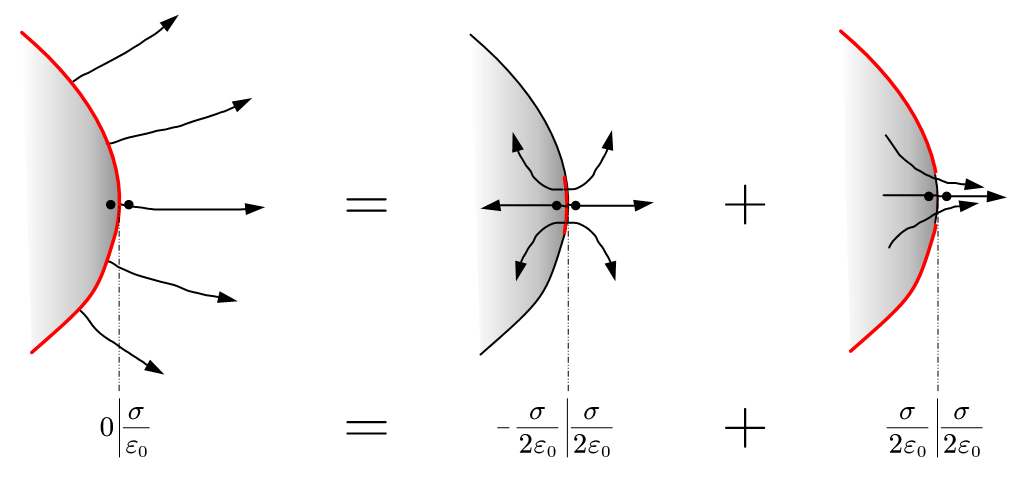
\includegraphics[width=0.6\textwidth]{image/7-2-3.png}
\caption{导体表面}
\end{figure}

但是正如上图所示,\,如果在十分接近表面的内外各取一点,\,就会发现如果只选取相对这两点足够大的一块面电荷(但又足够小以至于可以视作平面),\,它对面左右的电场强度只贡献以上值的一半.\,那么另一半必然由去掉这一块电荷的另外的部分所贡献.\,所以如果要讨论面上的场强,\,通过上一节的球体平均的理解方式,\,它就自然地被定义为内外场强和的一半,\,即:
\[\bs{E}=\frac{\sigma}{2\varepsilon_0}\bs{n}\]

对于导体静电平衡问题的计算求解,\,也包括模拟求解,\,本质上都建立在以下基本原理的基础上:

\begin{verse}
\emph{独立叠加原理}:\,静电平衡问题可以拆解为独立的在导体外部一个个连通区域内的静电边值问题.
\end{verse}

所谓的\emph{边值问题}(boundary value problem)本是偏微分方程的术语,\,在这里特指下面说的静电情况.\,每一种情况中,\,我们无需分析导体的内部的电荷,\,电场,\,电势.\,只需要求解外部的电场$\bs{E}(\bs{r})$和电势$\varphi(\bs{r})$.\,导体外部的电荷分布$\rho(\bs{r})$却是事先给定的.\,还给定了每一种导体表面的,\,要么是电势$V_i$(从而导体内部的电势也是这个值),\,把这种导体称作第一类导体,\,对应条件称为第一类边界条件;\,要么是给定了这个面上的总电量$Q_i$,\,把这种导体称作第二类导体,\,对应条件称为第二类边界条件.\,而每一个导体外部的区域的边界,\,就回到了各个导体的表面$\Sigma_1,\,\Sigma_2\cdots\Sigma_n,\,\Pi_1,\,\Pi_2\cdots\Pi_m$构成的集合.\,但是表面上的电荷分布也是事先不知道的.\,由于电荷,\,电场都可以从电势中得到,\,故只暂时考虑求电势,\,我们把静电边值问题整理一下:

\begin{verse}
\emph{已知}:\,导体外连通区域$D$以第一类导体表面$\Sigma_1,\,\Sigma_2\cdots\Sigma_n$和第二类导体表面$\Pi_1,\,\Pi_2\cdots\Pi_m$为边界.\,已知区域$D$内电荷分布$\rho$,\,已知第一类导体表面$\Sigma_i$上的电势$V_i$.\,已知第二类导体表面$\Pi_j$上的电量$Q_j$:
\[\partial D=\biggl(\bigcup_i \Sigma_i\biggr)\cup \biggl(\bigcup_j\Pi_j  \biggr) \]
\[\rho=\rho(\bs{r}) \quad,\quad \bs{r}\in D\]
\[\varphi(\bs{r})|_{\Sigma_i}=V_i \quad, \quad \int\limits_{\Pi_j}\nabla\varphi\cdot \ud \bs{S}=Q_j/\varepsilon_0 \quad, \quad \varphi(\bs{r})|_{\Pi_j}=C\]

\emph{未知}:\,导体表面电荷的具体分布$\sigma(\bs{r})|_{\Sigma_i,\,\Pi_j}$

\emph{待求}:\,$D$内的电势分布$\varphi(\bs{r})|_{D}$

\end{verse}


\begin{wrapfigure}[19]{o}[0pt]{7cm}
\vspace{-0.6cm}
\centering
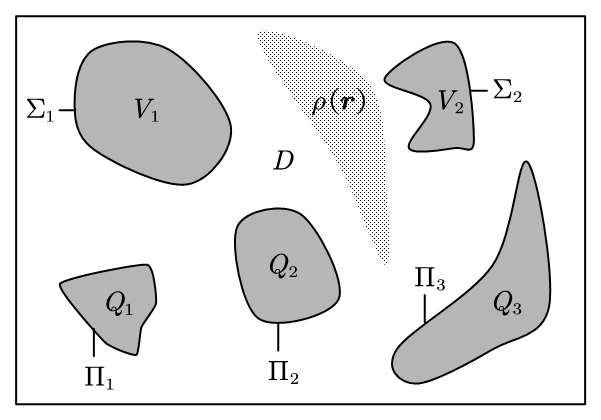
\includegraphics[width=7cm]{image/7-2-4.png}
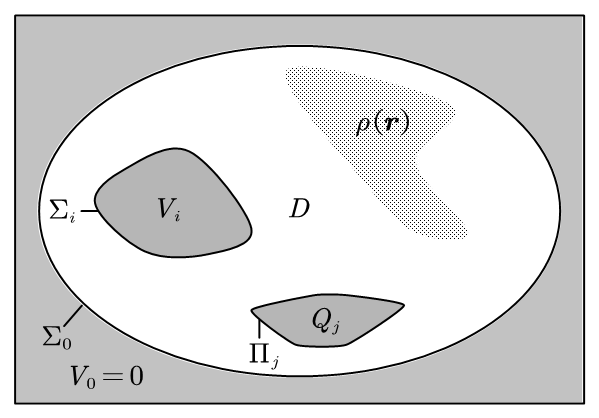
\includegraphics[width=7cm]{image/7-2-5.png}
\caption{边值问题}
\end{wrapfigure}
但是还要注意这种边值问题又分为\emph{外问题}(outside problem)和\emph{内问题}(inside problem)两类.\,外问题是区域$D$延伸到了无穷远,\,这种情况的边值问题提法就完全如上所述.\,但是内问题中区域$D$存在一个最外的表面$\Sigma_0$,\,它把整个$D$和其他所有金属表面与内部包含在其内部.\,$\Sigma_0$的外部亦是金属.\,对于内问题,\,我们很容易发现$\Sigma_0$上的总带电量为内部所有带电量的和的相反数,\,且仅仅由内部体系和它产生的电场线不会延伸到$\Sigma_0$外部.\,所以我们暂时可以以这一类问题中$\Sigma_0$上的电势为零点:
\[\varphi(\bs{r})|_{\Sigma_0}=0\]

这样所有已知未知的电势皆是相对$\Sigma_0$而言的电势差.


对于每一个具体的边值问题,\,指导我们求解的重要思想是\emph{广义叠加原理}(general superposition principle)和\emph{唯一性定理}(uniqueness theorem).\,从语义上看广义叠加原理显然与之前的单纯的叠加原理有着直接的联系.\,其实它更是来自于数学上具有线性结构的系统的解的叠加原理.\,这个叠加原理是这样表述的:
\begin{verse}
\emph{广义叠加原理}:\,两个边值问题如果$D,\,\Sigma_i,\,\Pi_j$一致.\,第一个问题具有第一类边界条件$V_{1i}$和第二类边界条件$Q_{1j}$和内部电荷分布$\rho_1(\bs{r})|_D$.\,第二个问题具有第一类边界条件$V_{2i}$和第二类边界条件$Q_{2j}$和内部电荷分布$\rho_2(\bs{r})|_D$.\,两个问题的解分别为$\varphi_1(\bs{r})|_D,\,\varphi_2(\bs{r})|_D$.\,则同样以$D$为区域,\,$\Sigma_i,\,\Pi_j$为$D$两类导体边界,\,但是以$V_{1i}+V_{2i}$和$Q_{1j}+Q_{2j}$为两类边界条件的问题的解一定是:
\[\varphi(\bs{r})=\varphi_1(\bs{r})+\varphi_2(\bs{r})\]
\end{verse}

这个定理的证明是显然的:\,首先$\varphi$作为一个边值问题的解,\,当且仅当它满足以下的一个全局条件和若干边值条件:
\[\nabla^2\varphi=-\frac{\rho}{\varepsilon_0}\]
\[\varphi(\bs{r})|_{\Sigma_i}=V_i \quad, \quad \int\limits_{\Pi_j}\nabla\varphi\cdot \ud \bs{S}=Q_j \quad, \quad \varphi(\bs{r})|_{\Pi_j}=C\]

那么既然$\varphi_1$和$\varphi_2$都是之前两个问题的解,\,这就意味着:
\[\nabla^2\varphi_1=-\frac{\rho_1}{\varepsilon_0} \quad,\quad \nabla^2\varphi_2=-\frac{\rho_2}{\varepsilon_0}\]
\[\varphi_1(\bs{r})|_{\Sigma_i}=V_{1i} \quad, \quad \int\limits_{\Pi_j}\nabla\varphi_1\cdot \ud \bs{S}=Q_{1j} \quad, \quad \varphi_1(\bs{r})|_{\Pi_j}=C\]
\[\varphi_2(\bs{r})|_{\Sigma_i}=V_{2i} \quad, \quad \int\limits_{\Pi_j}\nabla\varphi_2\cdot \ud \bs{S}=Q_{2j} \quad, \quad \varphi_2(\bs{r})|_{\Pi_j}=C\]

那么定义$\varphi=\varphi_1+\varphi_2$,\,它就自然也能满足:

\[\nabla^2\varphi=-\frac{\rho_1+\rho_2}{\varepsilon_0}\]
\[\varphi(\bs{r})|_{\Sigma_i}=V_{1i}+V_{2i} \quad, \quad \int\limits_{\Pi_j}\nabla\varphi\cdot \ud \bs{S}=Q_{1j}+Q_{2j} \quad, \quad \varphi(\bs{r})|_{\Pi_j}=C\]

从而就的确是新问题的一个解.\,但是这个解是否唯一?\,答案是肯定的.\,这就是著名的唯一性定理,\,可以这么表述:
\begin{verse}
\emph{唯一性定理}:\,如果同一个边值问题具有两个解$\varphi_1,\,\varphi_2$.\,那么$\varphi_1-\varphi_2= 0$.
\end{verse} 	 

其证明的核心思想是利用上一章介绍的第一格林等式\footnote{其实使用简单的``电荷发出电场线,\,沿电场线方向电势降低"的观点也是可以论证这个定理的.\,请读者思考过程.}.\,首先注意到如果$\varphi_1,\,\varphi_2$都是同一个边值问题的解.\,那么命$\varphi=\varphi_1-\varphi_2$就是以下边值问题的解:
\[\nabla^2\varphi=-\frac{\rho-\rho}{\varepsilon_0}=0\]
\[\varphi(\bs{r})|_{\Sigma_i}=0 \quad, \quad \int\limits_{\Pi_j}\nabla\varphi\cdot \ud \bs{S}=0 \quad, \quad \varphi(\bs{r})|_{\Pi_j}=C\]

上面这个等号右侧都是零的方程称作\emph{齐次方程}(homogeneous equation).\,那么问题就被转化为证明齐次方程的解必为零解.\,想起第一格林等式:
\[\nabla\cdot(\phi\nabla\psi)=\phi\nabla^2\psi+\nabla\phi\cdot\nabla\psi\]

同样是在$\phi,\,\psi$都取$\varphi$的情况:
\[\varphi\nabla^2\varphi=\nabla\cdot(\varphi\nabla\varphi)-(\nabla\varphi)^2\]

现在把$\varphi$就视作刚刚定义的$\varphi_1-\varphi_2$,\,并把这个公式运用于$D$中的任意一点,\,由于电势满足的条件$\nabla^2\varphi=0$,\,就有:
\[(\nabla\varphi)^2=\nabla\cdot(\varphi \nabla\varphi)\]

等号右侧会让人联想到奥-高定理.\,事实上如果把它应用到$D$:\,左右两侧就能化为:
\[\int\limits_D(\nabla\varphi)^2\ud V=\int\limits_D \nabla\cdot(\varphi \nabla\varphi)\ud V=\oint\limits_{\partial D}\varphi\nabla\varphi \cdot \ud \bs{S}=\oint\limits_{\scriptscriptstyle\left(\cup_i \Sigma_i\right)\cup \left(\cup_j\Pi_j  \right)}\cdots=\sum_i \oint\limits_{\Sigma_i}\varphi\nabla\varphi \cdot \ud \bs{S}+\sum_j \oint\limits_{\Pi_j}\varphi\nabla\varphi \cdot \ud \bs{S}\]

在第一类导体边界上,\,由于$\varphi=0$所以积分为零.\,在第二类导体边界上,\,首先$\varphi$也是常数所以可以提出到积分外面,\,即:
\[\oint\limits_{\Pi_j}\varphi\nabla\varphi \cdot \ud \bs{S}=C\cdot\oint\limits_{\Pi_j}\nabla\varphi \cdot \ud \bs{S}=C\cdot 0=0\]

从而得到恰好等号的右侧就是$0$.\,这就相当于证明了这个电势$\varphi$满足:
\[\int\limits_D(\nabla\varphi)^2\ud V=0\]

一个总是不小于零的$(\nabla\varphi)^2$,\,经过积分得到了零的结果.\,这就说明它恒等于零:
\[\nabla\varphi=\bs{0}\]

从而电势就是一个常数,\,由于在第一类边界条件上得取零,\,故只能是:
\[\varphi=0\]


以上两个原理是静电平衡问题能够被分析与解决的基础.\,以下几类问题中,\,区域$D$有高度对称性,\,且内部都没有电荷分布$\rho$,\,那么其解决甚至用不上这两个原理,\,下一节的电像法就非常依赖这两个原理了.\,不过这里的几类情况足以解决很多实际的问题:

\subsection{常见简单体系}

1.\,平行的无限大导体板

\begin{wrapfigure}[10]{o}[0pt]{9cm}
\vspace{-0.2cm}
\centering
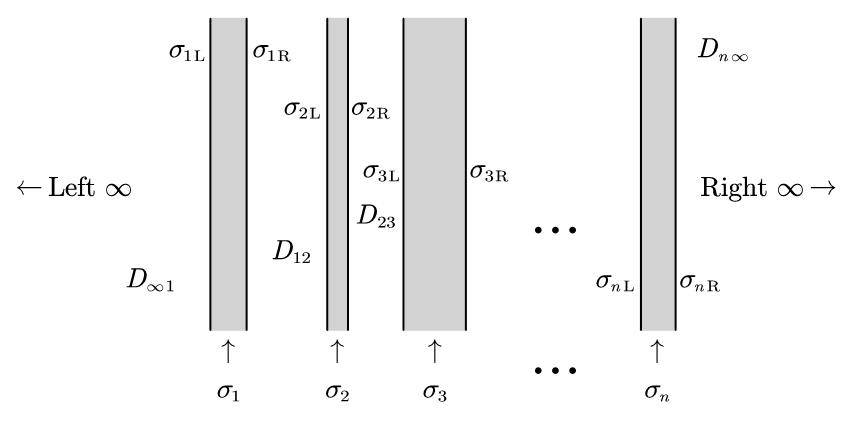
\includegraphics[width=9cm]{image/7-2-6.png}
\caption{平行板问题}\label{fig7-2-6}
\end{wrapfigure}
我们先考虑无限大的导体平面板,\,它可能具有一定的厚度.\,把这样的$n$块板子从左至右平行放置,\,如图\ref{fig7-2-6}.\,这样就把空间隔离为中间的$D_{12},\,D_{23},\,\cdots,\,D_{n-1\,n}$等区域.

我们没有必要严格写出这个问题的解.\,把这个体系的解需要满足的性质罗列出来会更实用.\,首当其冲地我们写出每一块板上的电量需要满足的关系.\,如果板非常薄,\,那么左右两侧的带电面密度$\sigma_{i{\rm L}}$和右侧$\sigma_{i{\rm R}}$就可以合成为统一的$\sigma_i$.\,那么以下两个特征是显著的:
\begin{enumerate}
\item $\sigma_{i{\rm R}}+\sigma_{i+1\,{\rm L}}=0$
\item $\sigma_{1{\rm L}}=\sigma_{n{\rm R}}=(\sigma_1+\cdots+\sigma_n)/2$
\end{enumerate}

而在第$i$与第$i+1$块板之间的区域$D_{i\,i+1}$内,\,如果研究场强,\,以向右为正.\,它应该满足两个关系:
\begin{enumerate}
\item[3.] $E_{i\,i+1}=\sigma_{i{\rm R}}/\varepsilon_0=-\sigma_{i+1\,{\rm L}}/\varepsilon_0$
\item[4.] $E_{i\,i+1}=(\sigma_1+\cdots+\sigma_i-\sigma_{i+1}-\cdots-\sigma_n)/2\varepsilon_0$
\end{enumerate}


请注意,\,在以上关系式中,\,$1,\,3$关系式仅仅依赖于上一节我们推出过的边界条件.\,是无条件成立的.\,但是$2,\,4$却无法从边界条件中推导出来.\,所以这两个式子的成立是有条件的:\,那就是整个体系``仅仅''由这些带电的板组成.\,事实上,\,如果把第$1$块板和第$n$向左向右平移到无限远,\,可以想象不改变板上的电荷分布也能保持静电平衡.\,但是这样中间就只剩下$2,\,3,\,\cdots,\,n-1$这些板,\,它们就可以造成典型的仅仅符合$1,\,3$而不符合$2,\,4$的带电体系.\,所以$2,\,4$的正确性要求``无穷远处不能有电荷分布''.\,此时我们可以通过叠加原理来解释$4$的正确性.\,又分过来通过$4$计算出来的电场强度用$3$来计算各板左右两侧的带电量.\,最后就能推导出$2$式来.

对于等式$2$,\,我们发现这实际上代表一种左右对称性:\,在这些所有板的外侧区域$D_{\infty 1},\,D_{n\infty}$观察,\,这些所有板等效于单块$\sigma_1+\cdots+\sigma_n$的板.\,从而左右的场强都是:
\[E_\infty=\frac{\sigma_1+\cdots+\sigma_n}{2\varepsilon_0}\]

\begin{wrapfigure}[10]{o}[0pt]{10cm}
\vspace{-0.2cm}
\centering
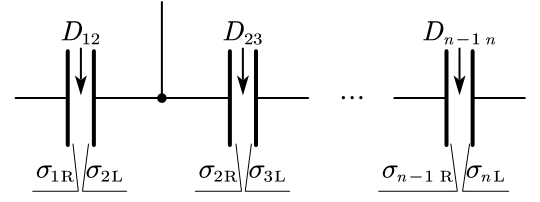
\includegraphics[width=10cm]{image/7-2-7.png}
\caption{电容器}\label{fig7-2-7}
\end{wrapfigure}
如果把上面的模型替换为电容器电路,\,各个区域$D$变成电容内部的场强区,\,而每一块导体板内部的区域被改成一根导线,\,并可以通过外界引入电量.\,那么需要注意,\,这个体系额外多了一个性质:\,\emph{一般情况下}各个电容器外侧的电量都一定是零.\,这是因为电容器初始状态必然不带电,\,而充放电过程是拟稳\footnote{即符合节点电流方程等,\,见之后章节的说明.}的,\,故两极板积累的电量必然相反.\,故按照上面的公式计算的$E_\infty$就是零.\,所以电容器极板外侧一般不允许有场强.\,除非遇到电容器中间被放置了外电荷的情况,\,比如在中间引入电压可以调控的栅极,\,对于这种``异型''电容的问题处理方法就又回到了之前我们说的四个结论上.

\vspace{0.5cm}
对于一个面积为$S$,\,极板间距为$l$的\emph{平板电容器}(parallel plate capacitor),\,正常工作的时候根据之前的结论,\,两板正对面带相反的电荷,\,电场线起始于带正电的板而终止于带负电的板.\,如果忽略其边缘效应,\,即$S\gg l$情况下,\,我们可以认为其去掉边缘以后的正对面积与$S$的相对误差非常小,\,电容就被定义为两板带正电或负电的绝对值与两板电势差的比值,\,它等于:
\[C=\frac{Q}{U}=\frac{\varepsilon_0S}{l}\]

\begin{wrapfigure}[12]{o}[0pt]{8.5cm}
\vspace{-0.5cm}
\centering
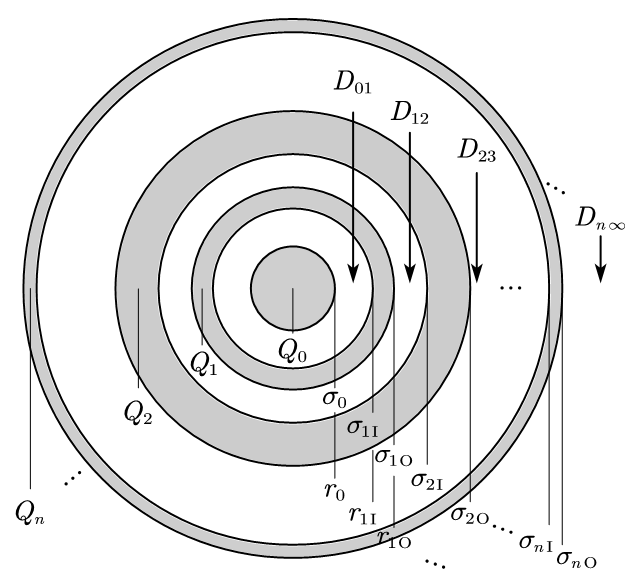
\includegraphics[width=8.5cm]{image/7-2-8.png}
\caption{球壳或柱壳}\label{fig7-2-8}
\end{wrapfigure}
当平板电容器带电时,\,其产生的能量可以通过静电能公式或计算外界做功,\,也可以用电场能量计算得到:
\[E=\frac{1}{2}CU^2=\frac{1}{2}QU=\frac{1}{2}\frac{Q^2}{C}\]

这个公式是普遍的,\,对任何符合上一个式子定义的电容都是成立的.

\vspace{1cm}
2.\,同心导体球与球壳

导体球与球壳反倒简单一些,\,它们面上的总带电量不存在发散的情况,\,而且也不需要考虑无穷远处的边界条件.\,用各内表面总带电量$Q_{\rm I}$和外表面带电量$Q_{\rm O}$描述,\,之前的四个条件现在也需要改写为:
\begin{center}\begin{minipage}{0.35\textwidth}
\begin{enumerate}
\item $Q_{i{\rm O}} +Q_{i+1\,{\rm I}}=0$
\item $Q_{n{\rm O}}=Q_1+\cdots+Q_n$
\item $E_{i\,i+1}=\dfrac{Q_{i{\rm O}}}{4\pi \varepsilon_0r^2}=-\dfrac{Q_{i+1\,{\rm I}}}{4\pi \varepsilon_0r^2}$
\item $E_{i\,i+1}=\dfrac{Q_1+\cdots+Q_i}{4\pi\varepsilon_0 r^2}$
\end{enumerate}
\end{minipage}\end{center}


两个球壳构成的电容器,\,如果内外球壳半径分别为$r_{\rm I}$和$r_{\rm O}$,\,那么电容为:
\[C=4\pi\varepsilon_0\frac{r_{\rm O}r_{\rm I}}{r_{\rm O}-r_{\rm I}}\]

\vspace{0.5cm}
3.\,共轴的导体圆柱与圆柱壳

我们先考虑无限长的圆柱.\,那么依然参考上图\ref{fig7-2-8}.\,圆柱带电应用单位长度的电量$\lambda$来描述,\,四个关系式变为:

\begin{center}\begin{minipage}{0.35\textwidth}
\begin{enumerate}
\item $\lambda_{i{\rm O}} +\lambda_{i+1\,{\rm I}}=0$
\item $\lambda_{n{\rm O}}=\lambda_1+\cdots+\lambda_n$
\item $E_{i\,i+1}=\dfrac{\lambda_{i{\rm O}}}{2\pi \varepsilon_0r}=-\dfrac{\lambda_{i+1\,{\rm I}}}{2\pi \varepsilon_0r}$
\item $E_{i\,i+1}=\dfrac{\lambda_1+\cdots+\lambda_i}{2\pi\varepsilon_0 r}$
\end{enumerate}
\end{minipage}\end{center}

两个柱壳构成的电容器,\,如果内外球壳半径分别为$r_{\rm I}$和$r_{\rm O}$,\,其长度为$l$且忽略边缘效应,\,即$l\gg r_{\rm O}>r_{\rm I}$那么电容为:
\[C=2\pi\varepsilon_0l\ln\frac{r_{\rm O}}{r_{\rm I}}\]

\section{电像法}

下面考虑两种实际的边值问题的解.\,第一种问题中区域$D$为半无限大空间,\,即,\,其边界为一个无限大导体的表面.\,第二种问题中区域$D$要么是一个球面外的延伸到无穷远的区域(外问题),\,要么是球面内的区域(内问题),\,不管哪种,\,区域边界都是导体的球面表面,\,只是前一种是外表面,\,后一种是内表面.

我们提供的方法为电像法.\,其意义是,\,先考虑一个较简单的,\,在空间中$\bs{R}$处放置一个点电荷$q$:
\[\rho(\bs{r})=q\delta(\bs{r}-\bs{R})\]

的情况下,\,边值问题的求解.\,其中$\delta(\bs{r}-\bs{R})$为\emph{狄拉克德尔塔函数}(Dirac delta function),\,读者大可以把它视作某物理量的某种极限化的密度分布的抽象\footnote{实则这样的广义函数数学上称作一种\emph{分布}(distribution),\,它是通过积分形式的运算定义的:
\[f(\bs{r}) \circ g(\bs{r}):=\int f(\bs{r})g(\bs{r})\ud V\]
\[\delta(\bs{r}-\bs{R})\circ g(\bs{r}):=g(\bs{R})\]
},\,例如物理量总值为$1$,\,分布在$\bs{R}=\bs{0}$附近的一个非常小的范围内,\,那么其密度就是:
\[\delta(\bs{r})=\begin{cases}
	+\infty &(\bs{r}=\bs{0})\\
	0	&(\bs{r}\neq \bs{0})
\end{cases} \qquad \&\quad \int\limits_{\rm Ball(\bs{0},\epsilon)} \delta(\bs{r})\ud V=1\]

那么此前的密度函数$\rho(\bs{r})=q\delta(\bs{r}-\bs{R})$就可以表示点电荷的电荷密度分布.

\subsection{半无限大空间的电像法}

下面考虑在无限大导体平板处建立坐标系,\,$z>0$就是待研究的$D$区域.\,现在在$\bs{R}$处放置一个正点电荷$q$,\,容易证明,\,由于导体板延伸到无穷远,\,所以导体板的表面自然成为第一类边界条件的表面且其电势为零$V=0$.\,表面上就会产生一个面电荷分布$\sigma(x,\,y)$.
\begin{figure}[H]
\centering
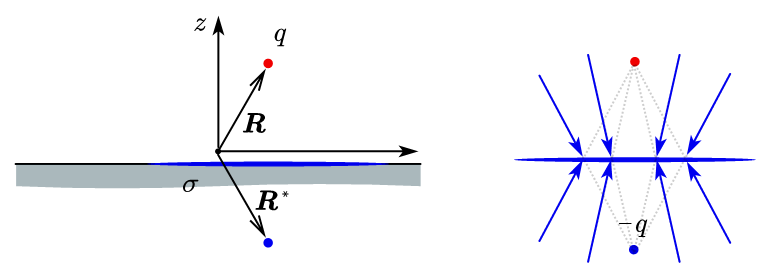
\includegraphics[width=0.7\textwidth]{image/7-2-9.png}
\caption{半无限空间的电像}
\end{figure}

见上图右,\,单独考虑这个面电荷产生的电场线,\,由于在$z<0$区域内为导体,\,合电场强度必然为零.\,故这个区域面电荷的电场线要与原来的$\bs{R}$处的$q$的电场线相抵消.\,故为指向$\bs{R}$处的汇聚的电场线.\,但是,\,由于这个面电荷产生的电场的上下的镜面对称性,\,这就导致我们可以直接证明它对$z>0$的$D$区域产生的电场线,\,实际上就相当于在$\bs{R}$的镜面对称点$\bs{R}^\ast$处放置一个\emph{像电荷}(image charge),\,值为$-q$而产生的电场.

从而$z>0$区域的电场,\,实际上就是由在$\bs{R}$的原电荷和在$\bs{R}^\ast$的像电荷共同产生的电场.\,或者说,\,满足以下方程的唯一解:
\[\nabla^2\varphi =-\frac{q\delta(\bs{r}-\bs{R})}{\varepsilon_0}\,(z>0)\quad ,\quad \varphi|_{z=0}=0\]

就是:
\[\varphi(\bs{r}) =\ke \frac{q}{|\bs{r}-\bs{R}|}-\ke \frac{q}{|\bs{r}-\bs{R}^\ast|}\]

那么我们如何求解下列更加普遍的第一类边值问题\footnote{第二类边值问题此时会有问题:\,首先导体面上的总电荷量就是上方的自由电荷量总值的相反数而不可以任意给定,\,而最终电势的结果也会产生一个未定常数的不确定性.}呢?
\[\nabla^2\varphi = -\frac{\rho(\bs{r})}{\varepsilon_0}\,(z>0)\quad ,\quad \varphi|_{z=0}=V\]

这个解答是简单的:\,就是对以上点电荷电像法的情形做叠加原理.\,我们把以上问题中,\,如果点电荷为单位电荷时,\,对应的解称作参数为$\bs{R}$处的\emph{格林函数}(Green function):
\[\delta(\bs{r}-\bs{R})\quad \longrightarrow\quad  \varphi(\bs{r})=\quad G(\bs{R},\,\bs{r})=\ke \left(\frac{1}{|\bs{r}-\bs{R}|}-\frac{1}{|\bs{r}-\bs{R}^\ast|}\right)\]

由于任意的电荷分布可以看成是点电荷的叠加,\,下式$\ud V$为$\bs{R}$改变对应的体积元:
\[\rho(\bs{r})=\int \rho(\bs{R})\delta(\bs{r}-\bs{R})\ud V\]

那么这个电荷分布产生的电势,\,就是各个点电荷的格林函数的叠加:
\[\rho(\bs{r})\quad \longrightarrow \quad \varphi(\bs{r})=\int  \rho(\bs{R})G(\bs{R},\,\bs{r})\ud V\]

这样在导体面上产生的电势依然是零,\,为了符合边界条件,\,只需要整体加上常数$V$,\,最终结果为:
\[\varphi(\bs{r})=V+\int \ke \left(\frac{1}{|\bs{r}-\bs{R}|}-\frac{1}{|\bs{r}-\bs{R}^\ast|}\right)\rho(\bs{R})\ud V\]

\subsection{球面外与球面内的电像法}

有了半无限区域的电像法求解边值问题做基础,\,我们对球面内外区域的边值问题的求解就有了线索.\,同样的,\,在球心处建立原点和坐标系,\,求解这两个问题的关键在于先求解以下两个最简单的第一类边值问题:
\[\nabla^2\varphi =-\frac{q\delta(\bs{r}-\bs{R})}{\varepsilon_0}\,(|\bs{r}|>a)\quad ,\quad \varphi|_{|\bs{r}|=a}=0\]
\[\nabla^2\varphi =-\frac{q\delta(\bs{r}-\bs{R})}{\varepsilon_0}\,(|\bs{r}|<a)\quad ,\quad \varphi|_{|\bs{r}|=a}=0\]

分别对应外问题和内问题.\,即下图左和右:
\begin{figure}[H]
\centering
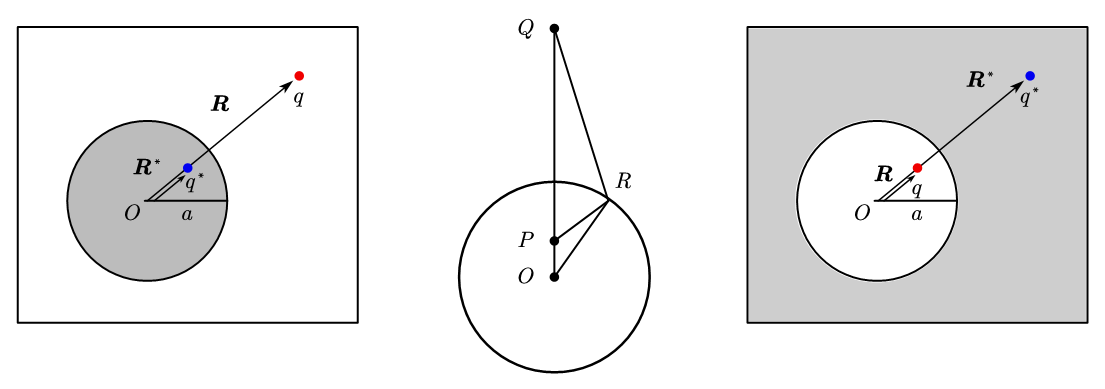
\includegraphics[width=0.8\textwidth]{image/7-2-10.png}
\caption{球面的电像}
\end{figure}

而以上两个问题的电像解,\,其实直接就都是:
\[\varphi(\bs{r}) =\ke \frac{q}{|\bs{r}-\bs{R}|}+\ke \frac{q^\ast}{|\bs{r}-\bs{R}^\ast|}\]

其中像电荷与原电荷在同一条半径上,\,且其大小$q^\ast$和到原点的距离$R^\ast$与圆的半径$a$分别满足:
\[RR^\ast=a^2\]
\[-\frac{q^\ast}{q}=\frac{a}{R}=\frac{R^\ast}{a}\]

证明这两个解的正确性的关键在于原电荷与像电荷的位置对圆是构成了一对反演点的关系.\,见上图中间的几何关系,\,不难证明:
\[\overline{OP}\cdot\overline{OQ}=a^2=\overline{OR}\quad \Rightarrow \quad \triangle OPR\sim \triangle ORQ\]

于是根据相似关系不难得到:
\[\frac{{\overline{OP}}^{1/2}}{\overline{PR}}=\frac{{\overline{OQ}}^{1/2}}{\overline{QR}}\]

所以只要让两个电荷分别位于$P,\,Q$处,\,且电荷量反号且大小之比为${\overline{OP}}^{1/2}:{\overline{OQ}}^{1/2}$,\,那么它们在$R$处的电势和就是零.\,实际上上面的电势解就是取了这样的两个电荷的电势的和,\,故就能满足原来的方程的边界条件,\,而这样的电势恰好在给定区域$D$内也能满足对应的微分方程:\,即$\nabla^2\varphi$只得到$\bs{R}$处电荷$q$.

这就证明了以上写出来的解是正确的.\,根据唯一性定理,\,它也是唯一的.

\vspace{0.5cm}
下面考虑在普遍的第一类和第二类边值问题下外问题的解.\,先考虑第一类边值问题,\,即:
\[\nabla^2\varphi = -\frac{\rho(\bs{r})}{\varepsilon_0}\,(|\bs{r}|>a)\quad ,\quad \varphi|_{|\bs{r}|=a}=V\]

同样的是利用以上解写出格林函数:
\[\quad G(\bs{R},\,\bs{r})=\ke \left(\frac{1}{|\bs{r}-\bs{R}|}-\frac{a/|\bs{R}|}{|\bs{r}-\bs{R}^\ast|}\right)\]

于是只需要写出下列积分,\,就可以满足问题前一半的拉普拉斯方程:
\[\int \rho(\bs{R})G(\bs{R},\,\bs{r})\ud V \]

这样一个势在边界上必然取零的值.\,为了使得最后的解满足边界条件,\,自然去思考叠加原理:\,让外界$\rho=0$且边界上具有电势$V$的电势显然为:
\[\varphi=\frac{VR}{r}\]

故,\,最后的解就是:
\[\varphi=\frac{VR}{r}+\int \ke \left(\frac{1}{|\bs{r}-\bs{R}|}-\frac{a/|\bs{R}|}{|\bs{r}-\bs{R}^\ast|}\right)\rho(\bs{R})\ud V\]

但是如果换为第二类边值问题:
\[\nabla^2\varphi = -\frac{\rho(\bs{r})}{\varepsilon_0}\,(|\bs{r}|>a)\quad ,\quad \int\limits_{|\bs{r}|=a}\nabla\varphi\cdot \ud \bs{S}=Q\;,\;\varphi|_{|\bs{r}|=a}=C\]

这就需要先考虑格林函数对应的势在边界上产生的总面电荷量,\,他其实就是像电荷的值:
\[\delta(\bs{r}-\bs{R})\quad \longrightarrow\quad  \int\limits_{|\bs{r}|=a}\nabla\varphi\cdot \ud \bs{S}=-\frac{a}{|\bs{R}|}\]

于是单独对格林函数进行积分得到的电势就使得面上带上电荷:
\[\rho(\bs{r})\quad \longrightarrow\quad \int\limits_{|\bs{r}|=a}\nabla\varphi\cdot \ud \bs{S}=-\int \frac{a}{|\bs{R}|}\rho(\bs{R})\ud V\]

那么通过叠加原理,\,为了使得面上电荷量变为$Q$,\,就需要引入一个电势:
\[\varphi=\ke \frac{Q+\displaystyle\int \frac{a}{|\bs{R}|}\rho(\bs{R})\ud V}{r}\]

综上,\,最后的解为:
\[\varphi =\ke \frac{Q+\displaystyle\int \frac{a}{|\bs{R}|}\rho(\bs{R})\ud V}{r}+\int \ke \left(\frac{1}{|\bs{r}-\bs{R}|}-\frac{a/|\bs{R}|}{|\bs{r}-\bs{R}^\ast|}\right)\rho(\bs{R})\ud V \]

球面外问题中,\,所有电势的结果都是$\rho(\bs{r})$和球面上的面电荷分布通过叠加原理产生的电势.

最后考虑内问题.\,我们介绍过,\,此时只有唯一的一种情况:\,即内表面取为电势为零的第一类边界条件.\,其问题表述和解必然为:
\[\nabla^2\varphi = -\frac{\rho(\bs{r})}{\varepsilon_0}\,(|\bs{r}|<a)\quad ,\quad \varphi|_{|\bs{r}|=a}=0\]
\[\varphi=\int \ke \left(\frac{1}{|\bs{r}-\bs{R}|}-\frac{a/|\bs{R}|}{|\bs{r}-\bs{R}^\ast|}\right)\rho(\bs{R})\ud V\]

这个电势就是内部的电荷$\rho(\bs{r})$和面上的感应面电荷共同对球内叠加产生的电势的和.\,对于球外的电势的叠加必然为零.

\subsection{几种其他情况*}

\vspace{0.2cm}
1. 立体谐函数
\vspace{0.2cm}

将一个中心在原点$\bs{r}=\bs{0}$,\,半径为$a$的球置于外场中讨论静电平衡为上一节中外问题的设置.\,但是上一节选择了在距离球心$R$处放置了一个点电荷.\,从而得到了球面在点电荷产生的外场下形成的格林函数$G(\bs{R},\,\bs{r})$.\,实用问题中通常把外场按照\emph{立体谐函数}(solid harmonics)在原点进行分解,\,类似于泰勒展开.\,只不过立体谐函数更适合于球坐标:
\[R_{lm}(\bs{r})=\sqrt{\frac{(l-m)!}{(l+m)!}}r^lP_{lm}(\cos\theta)e^{\ui m\varphi}\]
\[P_{lm}(x)=(-)^m(1-x^2)^{m/2}\frac{\ud^mP_l(x)}{\ud x^m}\]
\[P_l(x)=\frac{(-)^l}{2^ll!}\frac{\ud^l}{\ud x^l}(1-x^2)^l=\frac{1}{2^ll!}\frac{\ud^l}{\ud x^l}(x^2-1)^l\]

这样的复杂定义其实非常自然地缘起于球坐标下拉普拉斯方程的解.\,除了以上\emph{正规}(regular)部分,\,还有一组对应的在原点发散的\emph{非正规}(irregular)解:
\[I_{lm}(\bs{r})=\sqrt{\frac{(l-m)!}{(l+m)!}}r^{-(l+1)}P_{lm}(\cos\theta)e^{\ui m\varphi}\]

非正规解作为电势代表的场由放在原点的电荷,\,电偶极子乃至更高阶的对象产生.\,因为我们在原点放置了一个导体球, 所以它受到的外场不可能含有非正规成分.

以上完备谐函数组非常复杂,\,实际我们考虑的问题通常对球坐标$\varphi$的改变是对称的,\,例如球外点电荷对原点附近的外场,\,若以原点和点电荷的连线方向为极轴定义$\theta,\,\varphi$,\,那么这个外场就不含任何立体谐函数中$m\neq 0$的成分.\,此时仅考虑$m=0$的那些函数是完备的:
\[R_l(\bs{r})=\frac{1}{2^ll!}\cdot{r^l}\cdot\left(\frac{\ud}{\sin\theta\ud \theta}\right)^l\sin^{2l}\theta\]
\[I_l(\bs{r})=\frac{1}{2^ll!}\cdot\frac{1}{r^{l+1}}\cdot\left(\frac{\ud}{\sin\theta\ud \theta}\right)^l\sin^{2l}\theta\]

对于较小的$l$我们罗列若干对称立体谐函数:
\begin{table}[H]
\centering
\def\arraystretch{2}
\begin{tabular}{c|c|c}
\hline
l	&正规	&非正规 \\
\hline\hline
0	&$1$	&$\dfrac{1}{r}$\\\hline
1	&$r\cos\theta$	&$\dfrac{\cos\theta}{r^2}$\\\hline
2	&$\dfrac{r^2}{2}(3\cos^2\theta-1)$	&$\dfrac{1}{2r^3}(3\cos^2\theta-1)$\\\hline
3	&$\dfrac{r^3}{2}(5\cos^3\theta-3\cos\theta)$	&$\dfrac{1}{2r^4}(5\cos^3\theta-3\cos\theta)$\\\hline
4	&$\dfrac{r^4}{8}(35\cos^4\theta-30\cos^2\theta+3)$	&$\dfrac{1}{8r^5}(35\cos^4\theta-30\cos^2\theta+3)$\\\hline
$\vdots$&$\vdots$&$\vdots$\\\hline
\end{tabular}
\caption{对称立体谐函数表}
\end{table}

值得注意的是,\,正规的立体谐函数总是可以写成多项式的形式.\,如果以$\theta=0$的方向为$z$轴,\,那么$r\cos\theta=z,\,r^2=x^2+y^2+z^2$.\,这样就得到了对称情况下的\emph{谐和多项式}(harmonic polynomials),\,例如:
\begin{align}
R_0(\bs{r})=\mathcal{P}_0(x,\,y,\,z)	&=1\\
R_1(\bs{r})=\mathcal{P}_1(x,\,y,\,z)	&=z\\
R_2(\bs{r})=\mathcal{P}_2(x,\,y,\,z)	&=\frac{2z^2-(x^2+y^2)}{2}\\
R_3(\bs{r})=\mathcal{P}_3(x,\,y,\,z)	&=\frac{2z^3-3z(x^2+y^2)}{2}\\
R_4(\bs{r})=\mathcal{P}_4(x,\,y,\,z)	&=\frac{35z^4-30z^2(x^2+y^2)-3(x^2+y^2)^2}{8}\\
&\vdots
\end{align}

不难验证它们都会符合拉普拉斯方程:
\[\left(\frac{\partial^2}{\partial x^2}+\frac{\partial^2}{\partial y^2}+\frac{\partial^2}{\partial z^2}\right)\mathcal{P}_l(x,\,y,\,z)=0\]

就是这样的正规立体谐函数中的某项代表的电势,\,如果作为外场施加在置于原点的接地导体球上,\,应该得到怎样的静电平衡结果呢?\,首先我们明确这种场合下第一类边值问题表述为:
\[\nabla^2\varphi=0(|\bs{r}|>a)\quad ,\quad \varphi|_{|\bs{r}|=a}=0 \quad ,\quad \varphi|_{|\bs{r}|\to+ \infty}=\lambda R_l(\bs{r})\]

由于正规立体谐函数电荷摆放于无穷远处,\,而球面上感应电荷产生的电势在无穷远处影响一次反比于半径,\,故此时边界条件变成了一个\emph{渐进边值条件}(asymptotic boundary condition),\,它规定了半径趋近于无穷远时电势函数的变化趋势.

这个方程的解非常平庸地等于同阶的非正规立体谐函数与原来的正规谐函数的叠加:
\[\varphi(\bs{r})=\lambda R_l(\bs{r})+\mu I_l(\bs{r})\]

这是非常显然的.\,同阶的正规与非正规谐函数关于角度的部分变化趋势是一致的,\,为了满足在球面上电势为零的边值条件,\,我们只需要把半径取$a$并视作系数,\,再要求两个系数抵消,\,这只需要要求:
\[a^l\lambda+\frac{\mu}{a^{l+1}}=0\]

从而马上得到$\mu=-a^{2l+1}\lambda$.\,或者更简单地,\,我们把以下电势作为这一类问题的基础解:
\[\varphi=\frac{V_0}{2^l l!}\cdot\left[\left(\frac{a}{r}\right)^{l+1}-\left(\frac{r}{a}\right)^l\right]\cdot\left(\frac{\ud}{\sin\theta\ud \theta}\right)^l\sin^{2l}\theta\]

它代表怎样的电场呢?\,我们尤其关注$l=0,\,l=1$两种简单情况.\,此时电势为:
\[l=0\quad:\quad\varphi=\frac{V_0 a}{r}-V_0\]
\[l=1\quad:\quad\varphi=\frac{V_0 a^2\cos\theta}{2r^2}-\frac{V_0}{2a}r\cos\theta\]

作为外问题,\,$l=0$电势中的$-V_0$就必须理解为外场,\,而$\frac{V_0 a}{r}$则理解为球面上的感应电荷产生的场,\,很显然,\,这表示一个均匀带电的球面外的场,\,如图\ref{fig:7-1-23}左的第一种情况.

作为外问题,\,$l=1$电势中的$-\frac{V_0}{2a}r\cos\theta=-E_0 z$就必须理解为外场,\,而$\frac{V_0 a^2\cos\theta}{2r^2}=\frac{E_0 a^3\cos\theta}{r^2}$则理解为球面上的感应电荷产生的场,\,很显然,\,外场此时成为了$+z$方向的匀强电场$E_0\bs{e}_z$,\,而球面上的感应电荷产生的电势恰好与一个电偶极子产生的电势一致,\,电偶极矩为$\bs{p}=4\pi a^3\varepsilon_0\bs{E}_0$.\,如图\ref{fig:7-1-23}左的第二种情况.

\begin{figure}[H]
\centering
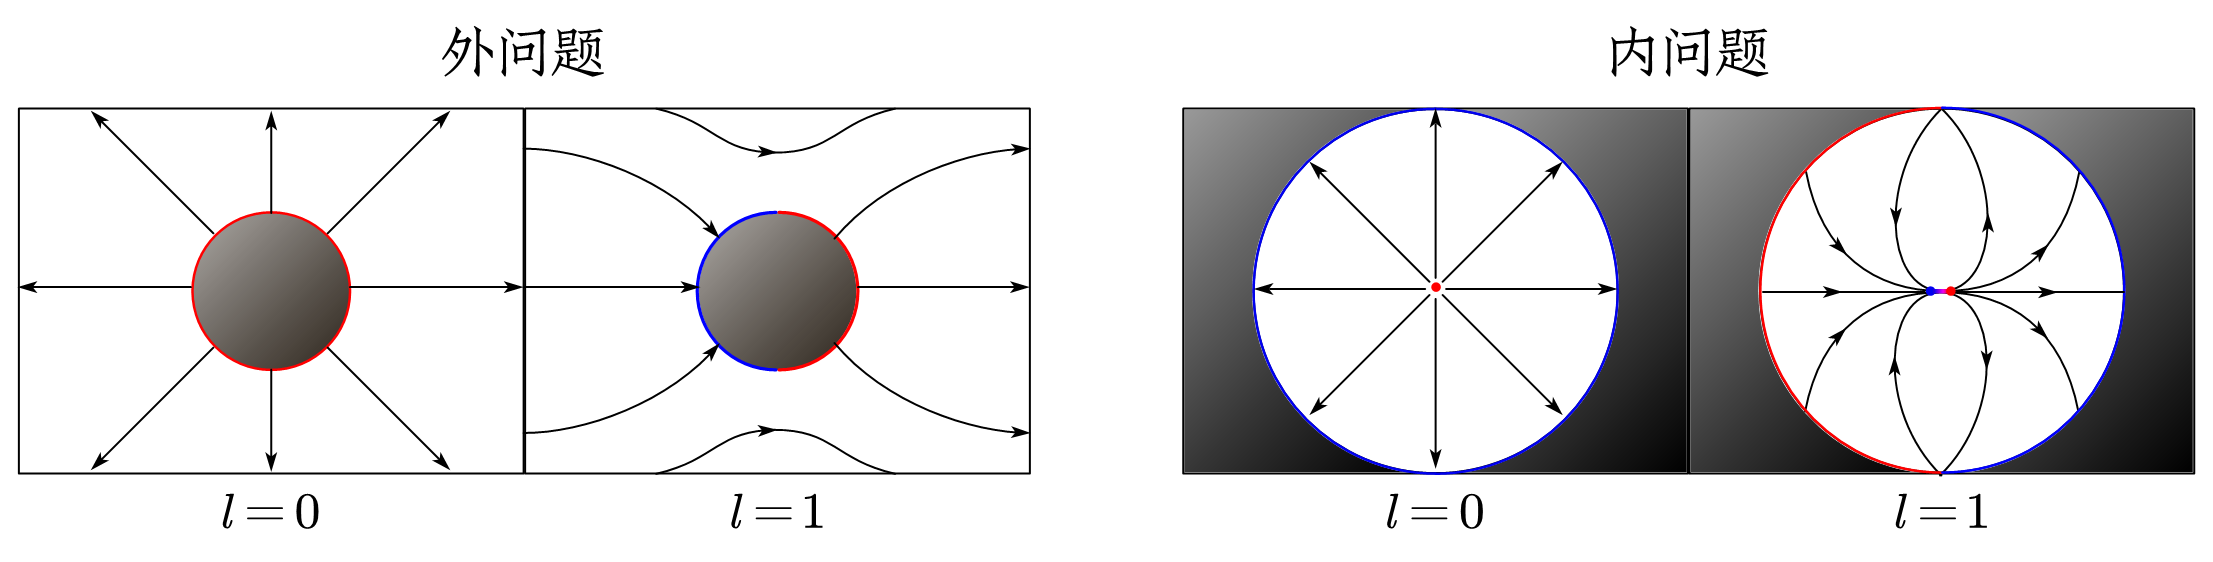
\includegraphics[width=0.9\textwidth]{image/7-1-23.png}
\caption{低阶立体谐函数静电平衡}\label{fig:7-1-23}
\end{figure}

有意思的是,\,这样的解也可以适用于内问题.\,此时球面上的感应电荷在原点产生的场应该展开为正规项,\,而非正规项对应放在球心的外电荷,\,此前的解两项将交换意义:

作为内问题,\,$l=0$电势中的$\frac{V_0 a}{r}$就必须理解为外场,\,而$-V_0$则理解为球面上的感应电荷产生的场,\,很显然,\,这相当于球心放了一个$Q=4\pi\varepsilon_0 aV_0$的点电荷造成的静电平衡,\,如图\ref{fig:7-1-23}右的第一种情况.

作为内问题,\,$l=1$电势中的$\frac{V_0 a^2\cos\theta}{2r^2}=\frac{p_0\cos\theta}{4\pi\varepsilon_0r^2}$就必须理解为外场,\,而$-\frac{V_0}{2a}r\cos\theta=-\frac{p_0}{4\pi\varepsilon_0 a^3} z$则理解为球面上的感应电荷产生的场,\,很显然,\,外场此时由$+z$方向的电偶极子$p_0\bs{e}_z$产生,\,而球面上的感应电荷产生的电势恰好是一个匀强电场$\bs{E}=\frac{\bs{p_0}}{4\pi\varepsilon_0 a^3}$.\,如图\ref{fig:7-1-23}右的第二种情况.

立体谐函数的意义在于,\,我们可以在原点附近去以球坐标的方式用正规的那些函数去展开一个电势,\,或者在一个球面外用非正规的那些函数去描写球面内的电荷体系产生的电势.\,故它天然地与多级展开挂钩.\,我们记得上一章我们用多级展开的思想来处理了偏移中心电荷的电势,\,多展开几项就是:
\[\ke \frac{q}{|\bs{r}-\bs{R}|}=\frac{q}{4\pi\varepsilon_0} \left[\frac{1}{r}+\frac{R\cos\theta}{r^2}+\frac{R^2(3\cos^2\theta-1)}{2r^3}+\frac{R^3(5\cos^3\theta-3\cos\theta)}{2r^4}+\cdots\right]\]

轻易就能发现,\,展开后各项,\,原来对应总电荷,\,电偶极矩,\,电四极矩,\,电八极矩等等,\,现在恰好就是一个个立体谐函数.\,它便是这样自然地产生于电势的多极展开中.\,个中原理在于以下展开式,\,又称\emph{勒让德多项式的母函数}(generatin function of Legendre polynomials):
\[\frac{1}{\sqrt{1-2xt+t^2}}=\sum_{n=0}^\infty P_l(x)t^l\]

而其中$P_l(x)$就是此前使用的\emph{勒让德多项式}(Legendre polynomials).\,我们此前是通过\emph{罗德里格公式}(Rodrigues' formula)引入它的:
\[P_l(x)=\frac{(-)^l}{2^ll!}\frac{\ud^l}{\ud x^l}(1-x^2)^l=\frac{1}{2^ll!}\frac{\ud^l}{\ud x^l}(x^2-1)^l\]

我们简要介绍一种通过母函数证明罗德里格公式的方法:

容易发现,\,根式$\sqrt{1-2xt+t^2}$出现在以下方程的解中:
\[tr^2-2r+2x-t=0\quad\Rightarrow\quad  r=\frac{1-\sqrt{1-2xt+t^2}}{t}\]

这样$t$也可以用$r$表示:
\[t=\frac{2(x-r)}{1-r^2}\]

但是$r$对$t$的泰勒展开为$r=x+(x^2-1)t/2+O(t^2)$.\,故重新命:
\[s=r-x=\frac{1-tx-\sqrt{1-2xt+t^2}}{t}=f(t)\]

这样用$s$表示$t$就是:
\[t=\frac{2s}{(s+x)^2-1}=g(s)\]

这样就存在两个互反函数$f\circ g=id$.\,且两者泰勒展开第一项都为一次项:
\[f(t)=f_1t^1+f_2t^2+\cdots\quad ,\quad f_1=\frac{x^2-1}{2}\]
\[g(s)=g_1s^1+g_2s^2+\cdots\quad ,\quad g_1=\frac{2}{x^2-1}\]

关于这样的函数有一个著名的\emph{拉格朗日反演定理}(Lagrange inversion theorem),\,如果用下角标表示泰勒展开的系数:
\[f_n=\frac{1}{n}\left(\frac{id}{g}\right)^n_{n-1}\]

写的更明确一点就是:
\[\left.\frac{\ud^n}{\ud t^n}f(t)\right|_{t=0}=\left.\frac{\ud^{n-1}}{\ud s^{n-1}}\left(\frac{s}{g(s)}\right)^n\right|_{s=0}\]

这个定理的证明如下:\,把$g(s)$代入$f$的泰勒展开式:
\[s=\sum_{m=1}^\infty f_m g^m(s)\]

两边对$s$求导数后乘以$s^n/g^n(s)$:
\begin{align*}
\left(\frac{s}{g(s)}\right)^n &=s^n\sum_{m=1}^\infty f_m \frac{\left[g^m(s)\right]'}{g^n(s)}\\
&=s^nf_n\frac{\left[g^n(s)\right]'}{g^n(s)}+s^n\sum_{m\neq n}^{1\to\infty}\frac{m}{m-n}f_m\left[g^{m-n}(s)\right]'\\
&=nf_ns^n\frac{g'(s)}{g(s)}+s^n\left(\sum_{m\neq n}^{1\to\infty}\frac{mf_m}{m-n} g^{m-n}(s)\right)'\\
&=nf_ns^n\frac{g_1+2g_2s+\cdots}{g_1s+g_2s^2+\cdots}+s^n\left(\sum_{l=-n+1}^{\infty}\frac{lf_{n+l}}{l} (g_1s+g_2s^2+\cdots)^l\right)'\\
&=nf_ns^{n-1}\left(1+\frac{g_2}{g_1}s+\cdots\right) +s^n\left(\cdots+\frac{c_{-2}}{s^2}+\frac{c_{-1}}{s}+c_0+c_1s+c_2s^2+\cdots\right)'\\
\end{align*}

后一项中,\,任意$s$的幂函数的导数都不会带来$s^{-1}$的结果项.\,故等号右侧唯一的$s^{n-1}$项就是$nf_ns^{n-1}$.从而可以提取左侧的$s^{n-1}$项系数得到右侧的$nf_n$.\,原命题得证.

将这个结果重新表示$f(t)$的泰勒展开,\,得到:
\[f(t)=\sum_{n=1}^{\infty}\frac{t^n}{n!}\left.\frac{\ud^{n-1}}{\ud s^{n-1}}\left(\frac{s}{g(s)}\right)^n\right|_{s=0}\]

现在,\,把此前的$g(s)$代入:
\begin{align*}
\frac{1-tx-\sqrt{1-2xt+t^2}}{t} &=\sum_{l=1}^{\infty}\frac{t^l}{2^l l!}\left.\frac{\ud^{l-1}}{\ud s^{l-1}}\left[(s+x)^2-1\right]^l\right|_{s=0}\\
&=\sum_{l=1}^{\infty}\frac{t^l}{2^l l!}\frac{\ud^{l-1}}{\ud x^{l-1}}\left(x^2-1\right)^l
\end{align*}

两边再次对$x$求导数:
\[-1+\frac{1}{\sqrt{1-2xt+t^2}}=\sum_{l=1}^{\infty}\frac{t^l}{2^l l!}\frac{\ud^{l}}{\ud x^{l}}\left(x^2-1\right)^l\]
\[\Rightarrow\quad \frac{1}{\sqrt{1-2xt+t^2}}=\sum_{l=0}^{\infty}P_l(x)t^l\quad ,\quad P_l(x)=\frac{1}{2^l l!}\frac{\ud^{l}}{\ud x^{l}}\left(x^2-1\right)^l\]


\begin{wrapfigure}[7]{o}[0pt]{6cm}
	\vspace{-0.6cm}
	\centering
	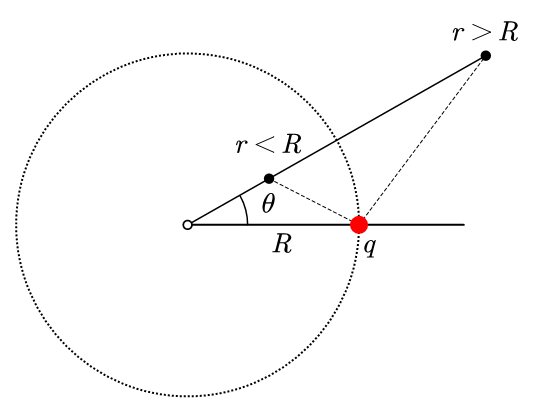
\includegraphics[width=6cm]{image/7-2-15.png}
	\caption{电势的勒让德展开}\label{fig:7-2-15}
\end{wrapfigure}
有了这个公式就可以把点电荷的电势进行展开,\,如图\ref{fig:7-2-15}所示,\,在半径$r$很小时原点附近应当视$x=r/R$展开为$r$的正规项,\,但是在半径$r$很大时的远方应当视$x=R/r$展开为$r$的非正规项:
\[\varphi=\frac{q}{4\pi\varepsilon_0}\frac{1}{\sqrt{R^2+r^2-2Rr\cos\theta}}=\begin{cases}
\displaystyle\sum_{l=0}^\infty \frac{qr^lP_l(\cos\theta)}{4\pi\varepsilon_0R^{l+1}}&(r<R)\\
\displaystyle\sum_{l=0}^\infty \frac{qR^lP_l(\cos\theta)}{4\pi\varepsilon_0r^{l+1}}&(r>R)
\end{cases}\]

\vspace{0.5cm}
现在让我们来尝试一下新的工具用来解球面内外放置点电荷的第一类边值问题的结果.\,对于外问题,\,在$r=a$处放置球面并接地,\,在$r=R$处放置点电荷$q$并沿其方向建立球极坐标.\,则球面感受到电势:
\[\varphi_q=\sum_{l=0}^\infty \frac{qr^lP_l(\cos\theta)}{4\pi\varepsilon_0R^{l+1}}=\sum_{l=0}^\infty \frac{qa^l}{4\pi\varepsilon_0R^{l+1}}P_l(\cos\theta)\left(\frac{r}{a}\right)^l\]

根据此前的讨论,\,球面上的感应电荷就会在$r>a$产生一个电势:
\[\varphi_{q^*}=-\sum_{l=0}^\infty \frac{qa^l}{4\pi\varepsilon_0R^{l+1}}P_l(\cos\theta)\left(\frac{a}{r}\right)^{l+1}=\sum_{l=0}^\infty \frac{(-qa/R)(a^2/R)^lP_l(\cos\theta)}{4\pi\varepsilon_0r^{l+1}}\]

恰好对应一个放置在$r=R^*$处的$q^*$产生的电势:
\[q^*=-\frac{a}{R}q\quad ,\quad R^*=\frac{a^2}{R}\]

内问题的验证在这里留给读者作为一个练习.

\vspace{1.2cm}
2. 正交坐标系
\vspace{0.2cm}

如果第一类边值问题的边界不再是平面或者球面,\,那么此时往往可以考虑建立特殊的坐标系来简化拉普拉斯方程.\,这是\emph{曲线坐标系}(curvelinear coodinates)在处理相关的问题上发挥了重要的用途.\,例如我们做一套坐标变换:
\[\bs{r}=\bs{r}(q_1,\,q_2,\,q_3)=x(q_1,\,q_2,\,q_3)\bs{i}+y(q_1,\,q_2,\,q_3)\bs{j}+z(q_1,\,q_2,\,q_3)\bs{k}\]

如果广义坐标$q_1,\,q_2,\,q_3$各自变化就可以让空间点沿曲线坐标系的坐标轴移动:
\[\dot{\bs{r}}=\frac{\partial \bs{r}}{\partial q_1}\dot{q}_1+\frac{\partial \bs{r}}{\partial q_2}\dot{q}_2+\frac{\partial \bs{r}}{\partial q_3}\dot{q}_3\]

\begin{wrapfigure}[12]{o}[0pt]{6.5cm}
	\vspace{-0.6cm}
	\centering
	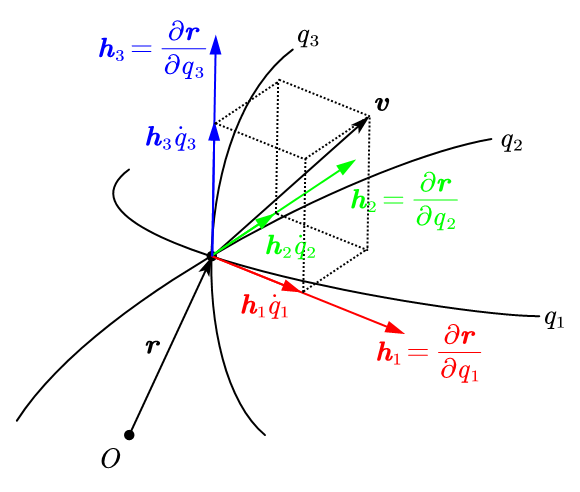
\includegraphics[width=6.5cm]{image/7-2-17.png}
	\caption{曲线坐标系}\label{fig:7-2-17}
\end{wrapfigure}
三个偏导数就可以看做\emph{拉梅系数}(Lam\`e coefficients),\,其实通常指他们的模:
\[h_1=|\bs{h}_1|=\frac{\partial \bs{r}}{\partial q_1}\quad ,\quad h_2=|\bs{h}_2|=\frac{\partial \bs{r}}{\partial q_2}\quad ,\quad h_3=|\bs{h}_3|=\frac{\partial \bs{r}}{\partial q_3}\]

如果三条曲线坐标轴总是互相垂直,\,即:
\[\bs{h}_i\cdot \bs{h}_j=0\quad (i\neq j)\]

那么这样的曲线坐标系称为\emph{正交坐标系}(orthogonal coordinates).\,接下来就会发现,\,正交坐标系下的静电平衡问题有着非常核心的地位,\,所以我们下面只研究正交坐标系的问题.\,在正交坐标系下的一个显著结论为如果广义坐标发生小的位移$\ud q_i$,\,那么产生的空间位移的模方可用三个位移的勾股定理合成:
\[\ud s^2=h_1^2\ud q_1^2+h_2^2\ud q_2^2+h_3^2\ud q_3^2\]

利用梯度和散度的几何定义式:
\[\ud f=\nabla f\cdot \ud\bs{r}\]
\[\oint \bs{F}\cdot \ud \bs{A}=\int \nabla \cdot \bs{F}\Delta V\]

再考虑到:
\[\ud r_i=h_i\ud q_i\]
\[\ud A_{i}=h_jh_k\ud q_j\ud q_k=h_1h_2h_3\ud q_i/h_i\;(i\neq j\neq k)\]
\[\ud V=h_1h_2h_3\ud q_1\ud q_2\ud q_3\]

这就得到:
\[\nabla^2\varphi=\nabla\cdot\nabla\varphi=\frac{1}{h_1h_2h_3}\frac{\partial}{\partial q_i}\left(\frac{h_1h_2h_3}{h_i^2}\frac{\partial \varphi}{\partial q_i}\right)\]

我们关心一种情况下体系的特殊静电平衡解存在的条件,\,这种解在求解区域内无任何外电荷(只在导体边界上存在自带电荷),\,且以比如$q_1$为唯一变量,\,而与$q_2,\,q_3$无关:
\[\varphi=\varphi(q_1)\quad :\quad \frac{\partial \varphi}{\partial q_2}=\frac{\partial \varphi}{\partial q_3}=0\]

代入拉普拉斯方程:
\[\nabla^2 \varphi=0\]
\[\Rightarrow \quad \frac{\partial}{\partial q_1}\left(\frac{h_2h_3}{h_1}\frac{\partial \varphi}{\partial q_1}\right)=0\]

这就等价于要求最后对$q_1$求偏导数前扩号内不含$q_1$.\,唯一可能的情形是:
\[\frac{h_2h_3}{h_1}=\frac{f(q_2,\,q_3)}{\partial \varphi/\partial q_1}=f(q_2,\,q_3)/g(q_1)\]

即:\,如果一个曲线坐标系的三个拉梅系数使得某坐标$q_1$对应的$h_2h_3/h_1$能够分离变量,\,即分解成$f(q_2,\,q_3)/g(q_1)$.\,则$\varphi(q_1)$形式的齐次拉普拉斯方程解存在且其值为:
\[\varphi=C_1+C_2\int g(q_1)\ud q_1\]

\begin{figure}[H]
\centering
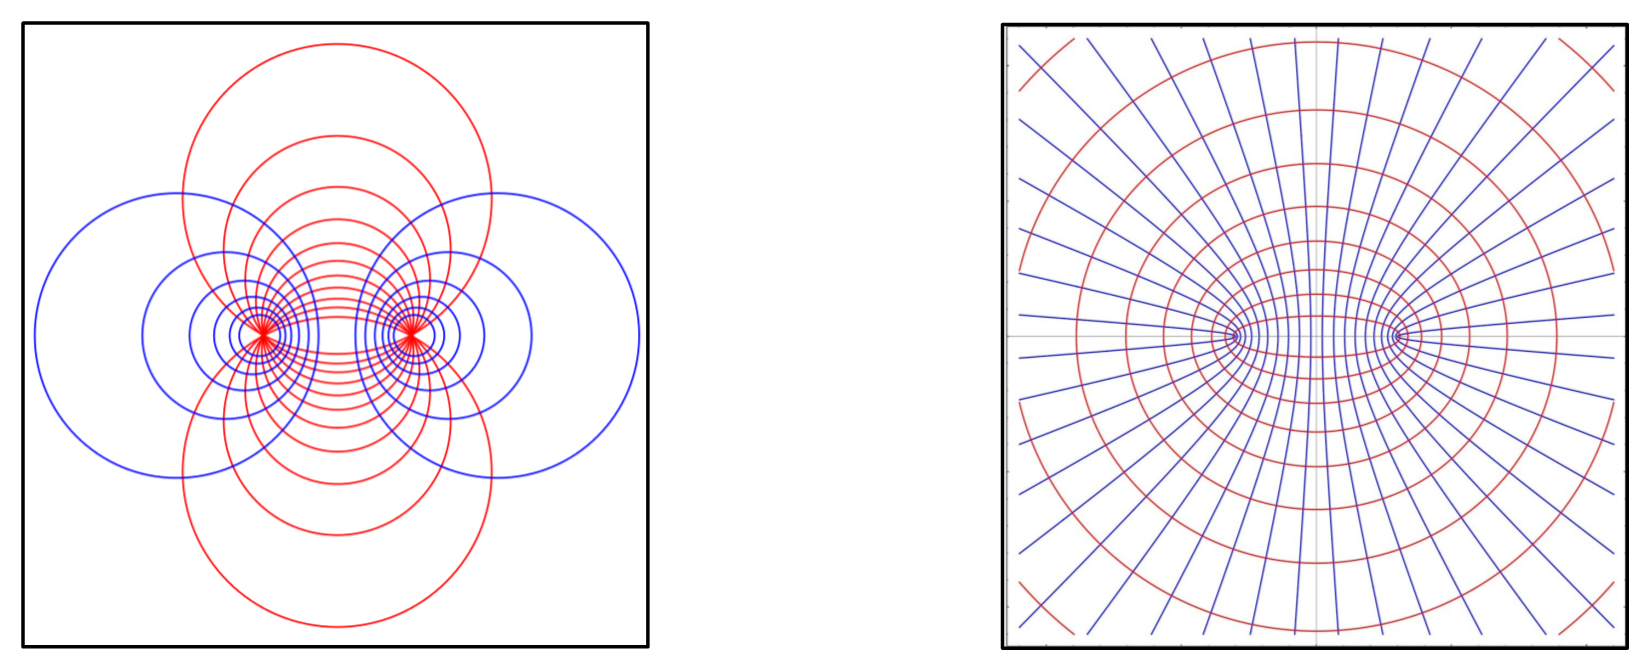
\includegraphics[width=0.7\textwidth]{image/7-2-19.png}
\caption{双极坐标与椭圆坐标}\label{fig:7-2-19}
\end{figure}

平面上有两套常见的正交曲线族.\,如图\ref{fig:7-2-19}所示,\,过平面上两点的圆族与到两点距离比值为常数的\emph{阿波罗尼斯圆}(Apollonian circle)族构成正交曲线族.\,而分别以两点为焦点的椭圆族与双曲线族也构成正交曲线族.\,对于这两个正交曲线族对应的正交坐标可以这样产生:\,考虑复平面$\mathbb{C}=\{x+\ui y|x,\,y\in \mathbb{R}\}$.\,平面上的点$(x,\,y)$用复数$z=x+\ui y$表示.\,那么取平面上两点$(\pm c,\,0)$,\,对应两个复数$\pm c$.

那么考虑函数$w(z)=u(z)+\ui v(z)$:
\[w=\ln\frac{z-c}{z+c}=\ln\frac{|z-c|}{|z+c|}+\ui\left[\arg(z-c)-\arg(z+c)\right]\]

从而:
\[u=\ln\frac{|z-c|}{|z+c|}\quad ,\quad v=\arg(z-c)-\arg(z+c)\]

那么$u-$坐标线,\,即$v$固定让$u$变,\,就是对两点张角固定的过两点的圆线(图\ref{fig:7-2-19}左的红线).\,而$v-$坐标线,\,即$u$固定让$v$变,\,就是到两点距离比为定值的圆线(图\ref{fig:7-2-19}左的蓝线).

从而反过来确定出用$w$计算$z$的方法:
\[z=c\tanh \frac{w}{2}\]

拆开实部虚部得到:
\[x=\frac{\sinh u}{\cosh u+\cos v}\quad ,\quad y=\frac{\sin v}{\cosh u+\cos v}\]




\subsection{格林互易定理}



\section{电介质}

之前介绍过,\,绝缘体只有考虑漏电或是大电场下击穿时,\,导电才得以发生.\,但这绝对不意味着忽略导电现象以后绝缘体对于静电场没有任何响应.\,这时发生的一个重要的现象为\emph{极化}(polarization).\,它会造成很多独特现象:\,从在头发上摩擦过的塑料笔杆对小纸屑的吸引\footnote{用金属屑的静电平衡也可以实现,\,不过金属屑密度大现象更不明显.},\,到电气工业大电容器的制作,\,更广义地说,\,在交变电场中介质的极化最终还能决定电磁波或光在介质中的传播,\,下一章我们将首次小小讨论以下这个问题.\,我们把明显能产生极化的介质称作\emph{电介质}(dielectrics).\,极化的含义可以从微观和宏观两个角度来考虑,\,背后涉及物理学的多个方面.\,我们分别进行讨论.\,最后揭示微观角度与宏观角度极化规律的联系.\,

\subsection{微观角度理解极化}

固体或晶体,\,尤其是离子晶体或部分共价晶体,\,每一个原子实际上本身就带电,\,其极化机理非常复杂,\,需要用到爱因斯坦,\,玻恩,\,黄坤等人的陆续完善的理论.\,或是放弃研究微观机理,\,通过宏观的方式引入唯象的描述方法.\,我们下面研究的主要是由原子,\,分子构成的气体或者液体的极化.

在这样的场合下,\,每一个单元被单独研究,\,原子或分子整体是没有电性的,\,但是正如之前所说的,\,下式决定的原子或分子的电偶极矩不必为零:
\[\bs{p}=\int \rho \bs{r} \ud V\]

如果从非量子的经典物理观点(包括半经典的玻尔模型)来看,\,即使简单如氢原子,\,看作轻的电子绕近似不动的质子做匀速圆周运动,\,每一个瞬时也会形成一个电偶极矩.\,但是它随时间快速转动而导致在静电场意义下其平均值为零.\,事实上,\,量子力学认为无论哪一个时刻,\,氢原子都处于电偶极矩沿任何方向概率都相等的\emph{定态}(stationary state),\,并没有在随时间演变.\.所以无论是从理论上来看还是从实际上来看,\,孤立氢原子基态下总是不体现电偶极矩的:
\[\overline{\bs{p}}=\bs{0}\]

具有这样性质的分子就称作\emph{无极分子}或\emph{非极性分子}(nonpolar molecule),\,反之则称作\emph{有极分子}或\emph{极性分子}(polar molecule)一般可以通过化学原理给出分子的成键和立体构型加以判断.\,例如${\rm CO}$分子和${\rm H_2 O}$具有极性而${\rm CO_2}$分子和${\rm CH_4}$则是无极的.

现在把无极分子放在外电场中,\,情况就会发生戏剧性的转变:\,把无极分子感受到的局部的电场视作匀强场,\,这个外场记做$\bs{E}'$.\,即使是简单如氢原子,\,其平均电偶极矩也不应当再视作零.\,这一个现象有若干解释方法:

\begin{enumerate}
\item 最唯象的解释方法把氢原子视作一个由劲度系数$k$的弹簧连接的作为正电负电中心的质点构成的体系,\,带电量为$\pm e$.\,但是忽略正负电荷之间的电相互作用力,\,只用去考虑受到的外力与等效电相互作用出来的线性弹性力的平衡,\,那么自然平衡时从负电荷到正电荷具有位移:
\[\bs{r}=\frac{e\bs{E}'}{k}\]

从而得到分子平均电偶极矩:
\[\overline{\bs{p}}=e\bs{r}=\frac{e^2}{k}\bs{E}'\]

\item 一个具有可证伪性的结果由以下考虑描述.\,通过量子理论的计算,\,把原子外的电子看作电子云,\,它是一个总电量为$-e$的连续电荷密度分布:
$$
\rho =\frac{-e}{\pi a_{0}^{3}}\ue^{-\frac{2r}{a_0}}
$$

其中$a_0=5.3\times 10^{-11}{\rm m}$为玻尔半径.\,进一步假设这个电荷分布为彻底刚性的.\,在外电场作用下,\,仅仅是原来在原点的质子现在位移到了$\bs{r}$处.\,质子对电子云的力就是电子云对质子的力,\,它与外电场力平衡.\,这样计算可以得到:
\[\bs{r}=\frac{3\pi\varepsilon_0 a_0^3}{e}\bs{E}\quad ,\quad \overline{\bs{p}}=3\pi\varepsilon_0 a_0^3\bs{E}'\]

\item 以上结果仅仅是与实验测量结果数量级一致,\,但是差了$6$倍,\,即实验结果表明:
\[\overline{\bs{p}}=18\pi\varepsilon_0 a_0^3\bs{E}'\]

这是因为上一个做法中认为电子云不会发生任何改变,\,反倒是质子位移了的做法不符合事实.\,正确的做法反而需要依然以质子为原点去解库仑场与弱匀强电场下电子的薛定谔方程的微扰解.\,这样才可以给出电子云的新分布.\,同样的计算也会带来著名的\emph{斯塔克效应}(Stark effect).\,即玻尔模型对应的第$n$能级(第$n-1$激发态)现在将分裂为$2n-1$个能级.\,进而影响谱线.

\end{enumerate}

不管用何种方式解释,\,以上现象就是第一种极化机理,\,称作\emph{位移极化}(distorsion polarization).\,它的结果为每一个分子产生了一个量子平均的电偶极矩,\,在弱场下这个电偶极矩应当正比于电场强度:
\[\overline{\bs{p}}=\alpha \bs{E}'\]

其中$\alpha$称作\emph{分子极化率}(molecular polarizability).\,它是表征微观极化难易程度的重要参数.\,对于位移极化,\,分子极化率是一个量子行为的结果,\,从氢原子的极化率就可以看出,\,因为玻尔半径$a_0$的计算依赖于普朗克常数的取值:
\[\alpha =18\pi\varepsilon_0 a_0^3=\frac{9(4\pi\varepsilon_0)^4\hbar^6}{2m_e^3e^6}=7.42\times 10^{-41} {\rm F\cdot m^2}\]
\vspace{1cm}

而对于有极分子,\,分子即使在没有外场作用时,\,由于其电荷分布本身就会造成一个电偶极矩,\,称作\emph{固有电偶极矩}(permanent dipole moment),\,我们记做$p_0$,\,但是由于无规则的热运动,\,其方向$\bs{e}$是随机的,\,所以作为每个分子的电偶极矩矢量$\bs{p}=p_0\bs{e}$的统计平均,\,其结果依然应当为$\bs{0}$:
\[\overline{\bs{p}}=\bs{0}\]

\begin{wrapfigure}[11]{o}[0pt]{6cm}
\vspace{-0.2cm}
\centering
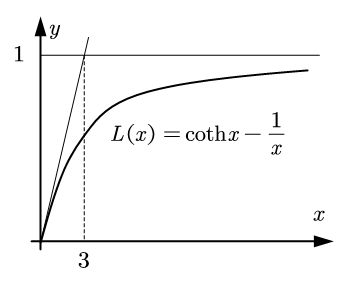
\includegraphics[width=6cm]{image/7-2-11.png}
\caption{郎之万函数}\label{fig7-2-11}
\end{wrapfigure}
现在施加外电场$\bs{E}'$以后,\,如果认为分子依然保持刚性,\,即$p_0$不变,\,但方向可以自由转动,\,则与电场保持同向的电偶极子的势能得到降低,\,电偶极子在动力学上倾向于与外电场同向排列.\,但是其热运动越剧烈,\,转动动能就越大,\,不同电偶极子相互影响就会使得其排列趋于杂乱无章.\,忽略可能的量子效应,\,由玻尔兹曼分布可以得到在温度为$T$时分子沿电场方向的平均电偶极矩:
\[\overline{p}=p_0\left({\rm coth}\,\frac{pE'}{kT}-1\middle/\frac{pE'}{kT}\right)\]

一般把上面这个函数称作\emph{郎之万函数}Langevin function),\,即:
\[\overline{p}=p_0 L\left(\frac{pE'}{kT}\right)\quad,\quad L(x)={\rm coth}\,x-\frac{1}{x}\]

这个函数的图像如\ref{fig7-2-11}所示.\,它有两条渐近线,\,分别对应两种具体的物理情形:

如果低温($T$很小)或者强场($E'$很大)但不至于漏电或击穿.\,使得宗量$x=pE'/kT\gg 1$,\,那么就使用水平$y=1$渐近线,\,即:
\[\overline{p}\approx p_0\]

对应几乎所有电偶极子都沿电场方向排列的\emph{饱和极化}(saturated polarization)情况.

如果高温($T$很大)或者弱场($E'$很小).\,使得宗量$x=pE'/kT\ll 1$,\,那么就使用原点切线$y=x/3$的渐近线,\,即:
\[\overline{p}\approx \frac{p_0^2}{3kT}E'\]

写成矢量式,\,我们发现与位移极化得到了相似的结果:
\[\overline{\bs{p}}=\alpha \bs{E}'\quad,\quad \alpha =\frac{p_0^2}{3kT}\]

这被称作\emph{郎之万-德拜定律}(Langevin-Debye law).\,同样地把$\alpha$称作分子极化率.\,而这种极化机理称作\emph{取向极化}(orientation polarization).\,取向极化的极化率是一个热学行为的结果,\,从极化率反比于温度这一点就可以看出来.

\vspace{1.5cm}

关于取向极化和位移极化我们总结以下几点:

一是要注意两者的不同:\,前者是外电场诱导产生或改变固有电偶极矩,\,是一个量子行为,\,几乎不依赖于温度.\,后者是外电场诱导固有电偶极矩选取优势方向,\,是一个热学现象,\,定性解释不依赖于量子特性.\,但是严格说来温度对前者也会有非常微小的影响,\,低温下量子特性对后者也会有不小的改变.

二是要注意两者可以同时出现:\,无极分子当然只能采取位移极化.\,但有极分子的取向极化和位移极化是并存的.\,所以分子极化率的完整计算方法为分别考虑两种极化方式带来的系数的和:
\[\alpha=\alpha_{\rm dis}+\alpha_{\rm ort}\]

三是要注意具体情况主要考虑哪一种极化方式:\,一般说来,\,有极分子的极化率中取向极化远大于位移极化的贡献\footnote{使分子转向导致的能量差小,\,使电子在不同能级间跃迁需要的能量差大,\,前者易后者难.},\,故有极分子的极化主要是取向极化.\,但是无极分子,\,位移极化就取代取向极化称为唯一需要考虑的极化因素了,\,故静电场下其分子极化率一般比有极分子要小一个量级.\,但是对于高频电场,\,\emph{弛豫时间}(relaxation time)成为了另一个需要考虑的重要因素.\,大约对于超过红外线频率的电场下,\,取向的改变就难以跟上电场的变化频率了,\,这导致介质的极化转而成为了电子的位移极化,\,考虑介质对光的色散和吸收都是基于这一点的.

\subsection{宏观角度理解极化}

之前章节已经介绍过极化强度$\bs{P}$的定义与相关的性质.\,宏观上的极化规律指的是,\,如果介质内部某点处局域地存在(平均意义下的)场强$\bs{E}$,\,那么该点就局域地产生一个极化强度$\bs{P}$,\,做为$\bs{E}$的响应函数:
\[\bs{P}=f(\bs{E})\]

这样的函数实际上或是应用上都不一定是线性的,\,但是在各向同性介质,\,弱场,\,低频的三个条件下,\,理论或实验都能给出线性的结果,\,一般写为:
\[\bs{P}=\chi_e \varepsilon_0 \bs{E}\]

这样$\chi_e$就是只与材料和环境(温度,\,压强)有关的,\,而与外加电场大小与方向无关的无量纲标量常数.\,称作\emph{极化率}(susceptibility).

类似于导体的静电平衡问题,\,介质的极化是如何达到平衡的?,\,这一个问题也应当动态地去思考:\,对比导体中的平衡条件$\bs{E}=\bs{0}$,\,介质中的上平衡条件也不过是一个最终才能达到的结果,\,达到平衡前的弛豫过程,\,等号不一定要成立.\,导体未平衡时,\,内部正是因为有电场才驱使电荷定向运动从而转移,\,从而电场才被改变,\,在改变中逐渐趋于零.\,那么介质也是类似:\,如果把一块未被极化的介质置于外电场$\bs{E}_0$中,\,一开始$\bs{P}=\bs{0}$将小于预期的$\chi_e \varepsilon_0 \bs{E}_0$值,\,那么极化就会慢慢发生,\,$\bs{P}$开始增大,\,位移极化和取向极化在逐渐发生,\,宏观看会产生\emph{极化电流}(polarization current),\,不难验证其电流密度为$\bs{J}_P=\partial \bs{P}/\partial t$.\,但是由于$\bs{P}$的变化,\,势必会在介质表面甚至内部产生极化电荷分布$\sigma_P,\,\rho_P$.\,这些电荷产生的场将部分抵消原来的外电场,\,称作\emph{退极化场}(depolarization field).\,于是$\bs{E}_0$也将动态的变化到最终的$\bs{E}$,\,使得以上平衡方程成立.\,这样极化强度就不再增加.

所以同样的以极化平衡条件$\bs{P}=\chi_e \varepsilon_0 \bs{E}$为出发点,\,应当期望可以类似于导体静电平衡那样得到有效的求解带电介质的静电平衡问题.\,但是由于平衡条件更复杂,\,我们的方法也需要进行改进.\,事实上不难验证改进的方法取$\chi_e\to+ \infty$就会退化为导体的情况.\,所以改进的方法反而更具有普遍性.

最核心的一点是引入辅助的\emph{电位移}(electric displacement)矢量来简化问题.\,这个矢量被定义为:
\[\bs{D}=\varepsilon_0 \bs{E}+\bs{P}\]

用$\bs{D}$的值反过来计算反映极化的$\bs{P}$,\,这会带来两个好处,\,第一是,\,极化规律的平衡条件被等价地写作:
\[\bs{D}=\varepsilon_0 \bs{E}+\chi_e \varepsilon_0 \bs{E}=\varepsilon_r \varepsilon_0 \bs{E}=\varepsilon \bs{E}\]

同样的$\varepsilon_r=1+\chi_e$也会作为一个基本常数,\,与原来的极化规律的结构复杂度一致.\,这个常数称作\emph{相对介电常数}(relative permittivity),\,其与真空介电常数$\varepsilon_0$的乘积$\varepsilon=\varepsilon_r \varepsilon_0$则称作\emph{绝对介电常数}(absolute permittivity)或简单称作\emph{介电常数}(permittivity).\,合理的极化率应当为正数,\,而根据相对介电常数的定义,\,它则要是大于$1$的正数.\,而介电常数的实用程度大于极化率的实用程度.

第二个关键的好处是,\,我们已经知道,\,$\bs{E}$与电荷通过高斯定理联系,\,而$\bs{P}$与极化电荷也可以通过高斯定理联系:
\[\nabla\cdot \bs{E}=\frac{\rho}{\varepsilon_0}\quad ,\quad \nabla\cdot \bs{P}=-\rho_P\]

代入刚才的电位移的定义马上就可以发现:
\[\nabla \cdot \bs{D}=\rho_f\]

即,\,电位移通过高斯定理联系的电荷就是``自由''电荷.\,这里的``自由''不是指导体中或导体表面的电荷,\,恰恰相反,\,如果把导体静电平衡问题中的导体也视作$\varepsilon_r\to+ \infty$的特殊电介质,\,这些电荷反倒要被排除.\,$\rho_f$的含义通过推导上式使用的关系式$\rho_f=\rho-\rho_P$就很容易看出来了,\,表示除去介质极化产生的面电荷或体电荷以外的一切电荷,\,一般都是置于介质外部区域的给定电荷,\,但对于介质情况它也可以分布在介质内.

对于带介质的静电平衡问题的求解就有了两种思路,\,第一种思路仅仅适用于比较简单的情况,\,这种情况不需要借助我们引入的电位移矢量$\bs{D}$就能得到结果.\,分别是把无限大块状介质和介质球放在匀强电场$\bs{E}_0$中的求解:

\begin{figure}[H]
\centering
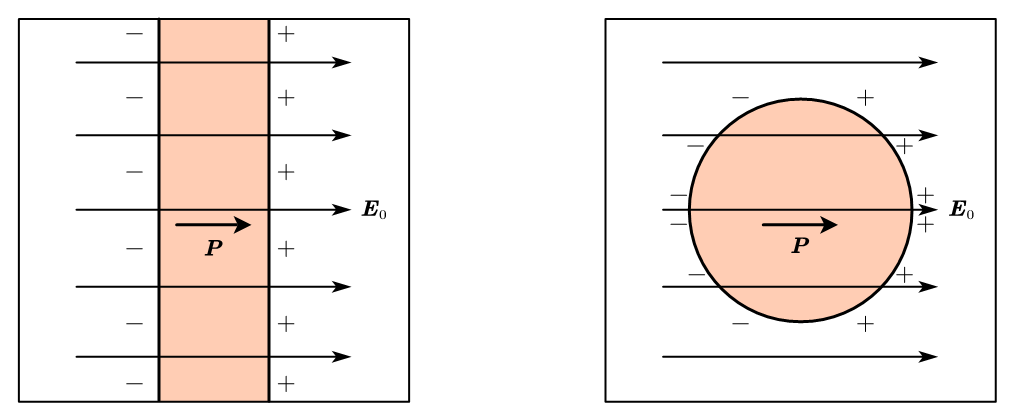
\includegraphics[width=0.6\textwidth]{image/7-2-12.png}
\caption{两种简单情况}
\end{figure}

这两个问题的核心在于大胆猜测介质内部是均匀极化的.\,设极化强度为$\bs{P}$.\,对于平板介质块,\,极化电荷在两侧产生的电荷面密度$\pm \sigma_P$就是:
\[\sigma_P=P\]

从而在介质内部形成的退极化场就是:
\[\bs{E}_P=-\frac{\bs{P}}{\varepsilon_0}\]

从而极化规律导致:
\[\bs{P}=\chi_e \varepsilon_0 \bs{E}=(\varepsilon_r-1)\varepsilon_0\left( \bs{E}_0 -\frac{\bs{P}}{\varepsilon_0}\right)\]

这就解出了平衡时的极化强度:
\[\bs{P}=\frac{\varepsilon_r-1}{\varepsilon_r}\varepsilon_0 \bs{E}_0\]

我们关心的是介质内部的电场强度:
\[\bs{E}=\bs{E}_0 -\frac{\bs{P}}{\varepsilon_0}=\frac{ \bs{E}_0}{\varepsilon_r}\]

这个结论很贴切地反应了$\varepsilon_r$的物理意义:\,它是简单的平板情况下介质对电场的削弱.\,故对于导体情况,\,内部电场强度在静电平衡时被削弱为零,\,故可以视作$\varepsilon_r\to +\infty$.

\begin{wrapfigure}[10]{o}[0pt]{7cm}
\vspace{-0.2cm}
\centering
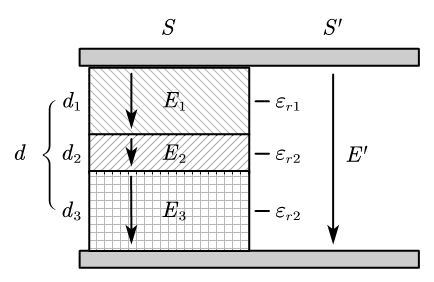
\includegraphics[width=7cm]{image/7-2-13.png}
\caption{电容器}\label{fig7-2-13}
\end{wrapfigure}
注意到这样的$\pm\sigma_P$在介质块外场强为零,\,故不影响外界.\,从而如果把多块介质块叠放,\,不同介质块就相当于按照不同的相对介电常数去削弱同一个电场.\,也就是说如图\ref{fig7-2-13}的三个介质块上方下方的导体板上的电荷面密度如果为$\sigma$,\,就会有:
\[E_0=\frac{\sigma}{\varepsilon_0}\quad ,\quad \varepsilon_{r1}E_1=\varepsilon_{r2}E_2=\varepsilon_{r3}E_3=E_0\]

但是要注意,\,这个$E_0$不一定要与旁边的空间中的$E'$相等,\,即在$S$和$S'$面上的电荷面密度没有必要是相等的,\,同一个表面的带电可以不均匀.\,而$E_i,\,i=1,\,2,\,3$也没有必要等于$E_0$,\,这不会与电场的环路定理矛盾,\,因为在介质块的边缘电场实际上已经不能视作匀强电场,\,而这一点作为边缘效应被我们忽略了.\,只有以下等势条件式是必须成立的:
\[E_1d_1+E_2d_2+E_3d_3=E'd=U\]

除了严格把以上量都解出来,\,我们讨论这个体系的静电平衡时经常会把它看做电容,\,每一个电容的性质和值由以下关系描述:
\[Q=CU\quad ,\quad C=\frac{\varepsilon S}{d}\]

注意电容器的并联等效电容应当满足直接求和的关系,\,串联反倒需要用电阻并联的方式来计算:
\[C_{\rm series}=C_1+C_2\quad ,\quad C_{\rm parallel}=C_1\parallel C_2=\frac{C_1C_2}{C_1+C_2}\]

于是上一个问题的总电容就是:
\[C=(C_1\parallel C_2\parallel C_3)+C'\]

现在让我们关心一下在三个介质中的电位移矢量,\,就会发现:
\[D_1=D_2=D_3=\varepsilon_0 E_0=\sigma\]

可以发现电位移与忽略电介质时的电场其实就差一个物理常数$\varepsilon_0$.\,它的存在可以理解为仅仅为了统一量纲.

\vspace{0.8cm}

现在让我们看介质球的极化问题.\,此时均匀的极化为球的表面带来的电荷面密度就变成了$\sigma_P=P\cos\theta$,\,而如上一章所述,\,这样的电荷分布带来的退极化场为:
\[\bs{E}_P=-\frac{\bs{P}}{3\varepsilon_0}\]

仅为块状情况的三分之一.\,可以想见,\,其极化会更加的强.\,事实上平衡方程与解变为:
\[\bs{P}=(\varepsilon_r-1)\varepsilon_0\left( \bs{E}_0 -\frac{\bs{P}}{3\varepsilon_0}\right)\quad \Rightarrow \quad \bs{P}=\frac{3(\varepsilon_r-1)}{\varepsilon_r+2}\varepsilon_0\bs{E}_0\]

那么球内的电场就被削弱到了:
\[\bs{E}= \bs{E}_0 -\frac{\bs{P}}{3\varepsilon_0}=\frac{3}{\varepsilon_r+2}\bs{E}_0\]

可见此时$\varepsilon_r$就没有体现出它的物理意义来:\,它并不能代表任意情况下介质对外加电场的削弱的比例,\,这里被削弱的比例变成了:
\[\epsilon=\frac{\varepsilon_r+2}{3}\]

从而这种情况下研究电位移表面上看上去没有意义:
\[\bs{D}=\varepsilon_0 \bs{E}+\bs{P}=\frac{3\varepsilon_r}{\varepsilon_r+2}\varepsilon_0\bs{E}_0\]

其实不然,\,下面我们来看带电介质的静电平衡问题的第二种思路,\,它也是普遍问题的处理思路,\,主要就是需要借助电位移矢量来考虑问题的.

\vspace{1cm}

首先,\,在同一种介电常数为$\varepsilon$的介质中,\,我们抛弃极化矢量$\bs{P}$,\,用电场强度$\bs{E}$和电位移$\bs{D}$可以完备地表达出极化平衡以后的场与荷(下面默认去除极化电荷,\,平衡的时候极化电荷的值是有唯一解的未知量)关系,\,它由三个关系构成:
\[\bs{D}=\varepsilon\bs{E}\]
\[\begin{cases}\;\nabla \cdot\bs{D}=\rho\\ \; \nabla \times\bs{E}=0\end{cases}\quad \text{或}\quad \begin{cases}\displaystyle\;\;\oint\limits_{\partial V} \bs{D}\cdot \ud \bs{A}=\int\limits_V\rho\ud V\\  \displaystyle\;\;\oint\limits_{\partial A} \bs{E}\cdot \ud \bs{l}=0\end{cases}\]

第一个式子称作电介质的\emph{本构方程}(constitutive equation).\,后两个式子就是介质中的高斯定律和环路定律.\,实际上还缺少一个势与它们的关系,\,势与场之间的关系不需要做任何改变:
\[\bs{E}=-\nabla \varphi\]

从而很容易得到势与荷之间的关系,\,现在变为:
\[\nabla^2\varphi=-\frac{\rho}{\varepsilon}\]

那么现在我们考虑电介质的静电平衡问题的表述方法.\,与导体静电平衡的区别在于,\,除了各真空区域$\varepsilon=\varepsilon_0$的电势分布待解以外,\,各个介质内部的电势分布也是待解的,\,我们甚至可以把外电荷引入介质的内部.\,这样我们索性就把空间按大块介质分成不同不相交的区域$D_i$的并:
\[\mathbb{R}^3=\bigcup_i D_i\]

每一个区域内部的介电常数为$\varepsilon_i$.\,而待解的电势为$\varphi_i$,\,如果该区域内有外电荷分布$\rho(\bs{r})$,\,则在介质内部需要满足:
\[\nabla^2\varphi(\bs{r})|_{\bs{r}\in D_i}=-\frac{\rho(\bs{r})}{\varepsilon_i}\]

但是凭以上方程不足以确定整个问题,\,一般还需要配合\emph{边界条件}(boundary relation).\,介质静电平衡问题的边界条件有它独特的重要性,\,一般会做如下表述:

\begin{wrapfigure}[8]{o}[0pt]{6cm}
\vspace{-0.9cm}
\centering
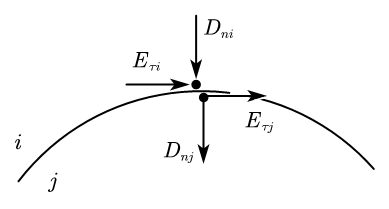
\includegraphics[width=6cm]{image/7-2-14.png}
\caption{边界条件}\label{fig7-2-14}
\end{wrapfigure}
如图\ref{fig7-2-14},\,在介质$i,\,j$的分界面上,\,把$i$指向$j$为正方向的场的法向分量的电位移记为$D_{ni},\,D_{nj}$.\,而切向分量以其自然方向为正方向的电场强度记做$E_{\tau i},\,E_{\tau j}$.\,如果面上没有外电荷,\,只有极化电荷,\,那么根据高斯定律和环路定律,\,容易得到:
\[D_{ni}=D_{nj}\quad ,\quad E_{\tau i}=E_{\tau j}\]

通常称作:\,\emph{法向电位移连续,\,切向电场强度连续.}

但是面上如果有$\sigma_{ij}$的外电荷,\,第一个式子就必须改为:
\[D_{nj}-D_{ni}=\sigma_{ij}\]

用这样的方程来确定平板电容器或其他具有高对称性电容器中的场分布非常方便.\,即使是之前的球在匀强电场中极化的问题,\,抛弃极化矢量而取而代之利用电位移也不会造成困难.\,此时我们假设表面上的电荷分布为$\sigma=\sigma_0 \cos\theta$.\,那么对面内面外产生的退极化场场强为:
\[\bs{E}_P=\begin{cases}\displaystyle\;-\frac{\sigma_0	}{3\varepsilon_0} \bs{e}&(r<R)\\\displaystyle \; \ke \frac{2p\cos\theta }{r^3}\bs{e}_r+\ke \frac{p\sin\theta }{r^3}\bs{e}_\theta&(r>R)\end{cases}\]

其中$p=4\pi\sigma_0 R^3/3$.\,现在取在$\theta=0,\,r=R$处的分界面,\,将退极化场与外场叠加,\,得法向内外场强分别为:
\[E_1=E_0-\frac{\sigma_0	}{3\varepsilon_0}\quad ,\quad E_2 =E_0+\ke \frac{2p}{R^3}=E_0+\frac{2\sigma_0	}{3\varepsilon_0}\]

再由法向电位移连续条件,\,即得到:
\[\varepsilon_r \varepsilon_0 E_1=\varepsilon_0 E_2\quad \Rightarrow \quad \sigma_0=\frac{3(\varepsilon_r-1)}{\varepsilon_r+2}\varepsilon_0 E_0\]

代入之前的电场表达式就得到了平衡时的场强分布.

\vspace{1cm}

但是含介质问题的静电平衡问题难度有甚于导体的静电平衡问题:\,在导体静电平衡问题中我们发展了格林函数法,\,并对区域$D$的边界为平面和球面两种情况分别引入了电像法.\,但是对于介质问题,\,可以证明平面情况依然可以使用电像法,\,但是球面的静电平衡问题外电荷已经不存在单个的简单的电像.\,此时原则上静电平衡的求解需要用到偏微分方程求解的通用思路,\,这已经超出本教材的范围,\,在此不再加以介绍.


\subsection{微观与宏观的联系}

我们已经得到微观和宏观的极化规律并使用后者解决了一部分问题:
\[\overline{\bs{p}}=\alpha \bs{E}'\quad ,\quad \bs{P}=\chi_e \varepsilon_0\bs{E}\]

当然如果单个分子的平均电偶极矩为$\overline{\bs{p}}$,\,而这些分子以数密度$n$组成介质,\,那么介质的极化强度满足以下关系式也是正确无误的:
\[\bs{P}=n\overline{\bs{p}}\]

但因此而认为微观的分子极化率是通过以下关系式确定宏观的极化率$\chi_e$的话就不够准确了:
\[\chi_e=\frac{n\alpha }{\varepsilon_0}\]

这是因为$\bs{E}'$和$\bs{E}$略有区别.\,但是我们先指出,\,以上做法对于稀疏的材料,\,比如气体,\,通常是足够准确的了.\,但是一旦分子稠密起来,\,比如低温下的液氦或是分子晶体固体,\,就必须考虑$\bs{E}'$和$\bs{E}$的区别.\,前者是造成分子极化的场强,\,而后者则是在宏观小,\,微观大尺度下平均化的局域场强.\,两者的区别实际上就在于偶极子自己的场强在前者计算中需要略去,\,因为自己的场强不可能极化自己.\,而后者则需要加以考虑.\,定量上的差值实际上我们在上一章末也进行过计算,\,关系式为:
\[\bs{E}'=\bs{E}+\frac{\bs{P}}{3\varepsilon_0}\]

这样就得到更准确的关系式:
\[\chi_e=\frac{n\alpha}{\varepsilon_0-n\alpha/3}\]

可见,\,如果$n\alpha\ll \varepsilon_0$,\,那么之前的近似计算法就可以适用,\,此时总是有$\chi_e\ll 1$,\,从而只会得到$\varepsilon_r\approx 1$介质的介电特性与真空区别不大.\,所以对于所有介电特性明显的电介质,\,实际的联系微观分子极化率与宏观极化率的公式必然是以上式子,\,或者写为相对介电常数:
\[\varepsilon_r=\frac{\varepsilon_0+2n\alpha/3}{\varepsilon_0-n\alpha/3}\]

这两个公式称为\emph{克劳修斯-莫索蒂关系}(Clausius-Mossotti relation).\,我们对于稀薄介质的判定条件进一步加以说明.\,如果采用氢原子的位移极化模型,\,我们就知道$\alpha =18\pi \varepsilon_0 a_0^3$,\,代入条件$n\alpha\ll \varepsilon_0$就得到了:
\[na_0^3\ll 1\]

如果把每个分子占据的体积近似为$a_0^3$,\,这就是说,\,单位体积内被分子占据的体积必须是个小量,\,主要的体积必须是被真空占据才能称作``稀薄''.\,这一点也符合物理的直觉.\,但是要注意,\,如果考虑取向极化,\,分子极化率要大一个量级,\,那么就要求$n$更小一个量级才能符合``稀薄''的条件.

\section{再议静电能}

导体静电平衡时的总静电能计算并不会带来任何问题.\,之前的用荷与势的公式和用场的计算公式依然适用:
\[I=\frac{1}{2}\int\limits_{V}\rho \varphi \ud V=\int\limits_{V}\frac{1}{2}\varepsilon_0\bs{E}^2\ud V\]

唯一要注意的问题是别在使用电像法的场合,\,把像电荷也代入第一个电荷乘电势的公式去计算了.\,这很可笑,\,第一可笑是即使出现了像电荷,\,它也仅仅是作为一种替代:\,用来替代某一部分感应电荷在某一特定区域产生的场强与电势.\,但绝对不是说这个虚假的电荷和它那个位置的实际的电势会对这个像电荷产生一个实际的能量.\,第二可笑是因为在更多的静电平衡问题中原则上没法用电像法,\,就更加不存在使用上面的积分计算静电能时没有考虑像电荷上的能量的问题了.

还有一个细节可以简化:\,实际上导体静电平衡问题中除了第一类或第二类区域,\,现在统一记为$D_i$中可以有$\rho(\bs{r})$分布以外,\,其余部分就是各个导体,\,每一个导体都等势,\,故具有带电量$Q_j$和电势$V_j$.\,那么总的静电能就可以更具体地表达为:
\[I=\sum_i \frac{1}{2}\int\limits_{D_i}\rho \varphi \ud V+\sum_j \frac{1}{2}Q_iV_i\]

如果实际电荷分布实际由微观的点电荷形成,\,那么在平均场意义下的上式应当代表所有点电荷之间的相互作用能的和.\,而点电荷的自能并不包含在上式中:\,它一般也不会改变.

但是如果遇到电介质极化的情况,\,问题就大不相同了!\,因为此时伴随着分子的极化,\,分子内部的能量也会改变.\,位移极化改变了分子的自能是不言而喻的.\,但是取向极化何以改变分子内部的自能?\,分子仅仅是在外电场下选取了优势方向而已.\,事实上,\,注意到极化率是温度的函数,\,就非常容易理解,\,此时有效的能量其实不是真正的系统内能,\,而是热力学理论中的自由能,\,它代表体系能量最低原理与熵最大原理的一种平衡:
\[F=U-TS\]

当分子取向杂乱无章时,\,极化强度$\bs{P}=\bs{0}$,\,此时熵最大,\,自由能最小.\,可以取为自由能的零点.\,但是一旦产生极化,\,$\bs{P}\neq\bs{0}$,\,此时熵减小,\,自由能就因此而增加.

这样就不难理解,\,讨论介质极化时,\,此时的能量(自由能)应当具有四个组成部分:
\begin{enumerate}
	\item 非宏观静电形式的,\,形成极化导致的\emph{极化能}(polarization energy).
	\item 单纯看介质极化自己产生的,\,介质内外的电场能,\,即介质自己的静电自能.
	\item 不考虑介质时其他电荷产生的全空间的电场能,\,即其他电荷分布的静电自能.
	\item 介质与其他电荷之间的静电相互作用能.
\end{enumerate}

其中后三个部分构成了我们之前意义上的``静电能''.\,但是它并不是能量的全部.\,考虑一个能量守恒的过程时,\,应当有外界做的功等于体系内部所有能量的变化.\,如为一个电容器充电的过程.\,很容易发现,\,如果介质内部采取取向极化,\,在一个等温的极化过程中介质是要向外界放热的,\,因为体系的熵在降低.\,故外界需要做的功,\,并不是要与体系的内能挂钩,\,而是直接与自由能挂钩:
\[W=\Delta U-Q=\Delta U-T\Delta S=\Delta F\]

所以从这个意义上说,\,我们此时定义的静电能,\,应当包括第一项极化能,\,而直接就是指自由能:
\[I=F\]

我们从平板电容器的极化来思考其表达式,\,因为这种情况场是简单的匀强场,\,而且区域限制在简单的长方体的内部.\,我们不妨预先假设,\,极化能的能量密度应当为极化强度的二次函数:
\[w_p=\frac{1}{2}\alpha \bs{P}^2\]

做这个假设的原因是因为自由能必然可以对$\bs{P}$泰勒展开,\,而空间的各向同性决定了它必然不含一阶的项(一维情况就是必然是偶函数),\,那么处于弱场近似可以忽略高阶项.\,其实待会也可以发现,\,这是唯一能够得到之前的极化规律的能量密度的取法.

那么在电容器完成极化后,\,真正的静电能,\,就应当为上式代表的极化能与后三项代表的之前意义上的``静电能''的和,\,其能量密度为:
\[w=w_p+w_0=\frac{1}{2}\alpha \bs{P}^2+\frac{1}{2}\varepsilon_0 \bs{E}^2\]

此时我们可以将介质的极化看作是一种自由能最小的结果:\,需要将外场$\bs{E}_0$视作一种不变的约束,\,而极化强度被视作自由能中的变量,\,在极化平衡时应当有以下自由能密度函数最小:
\[w=\frac{1}{2}\alpha \bs{P}^2+\frac{1}{2}\varepsilon_0 (\bs{E}_0-\frac{\bs{P}}{\varepsilon_0})^2\]

那么由导数为零的方式得到:
\[\alpha\bs{P}=\bs{E}_0-\frac{\bs{P}}{\varepsilon_0}\]

对比之前的极化规律,\,我们就非常容易看出来:
\[\alpha=\frac{1}{\chi_e\varepsilon_0}\]

从而得到极化能量密度的表达式:
\[w_p=\frac{\bs{P}^2}{2\chi_e\varepsilon_0}\]

这一点我们在用稀薄气体模型配合位移极化中的最唯象的弹簧模型进行一个验证.\,位移极化使得每个弹簧偏离平衡位置$\bs{r}$以后,\,弹簧势能造成的能量密度就是极化能的本质:
\[w_p=n\cdot\frac{1}{2}k\bs{r}^2\]

再结合宏观极化强度,\,微观电偶极矩与位移值三者的关系:
\[\bs{P}=n\bs{p}=ne\bs{r}\]

得到:
\[w_p=\frac{\bs{P}^2}{2ne^2/k}\]

而由之前讨论过的平衡方程得到分子极化率:
\[\alpha=\frac{e^2}{k}\]

从而宏观极化率,\,在稀薄条件下为:
\[\chi_e=\frac{n\alpha }{\varepsilon_0}\]

把上两式去代换之前的极化能,\,就得到了:
\[w_p=\frac{\bs{P}^2}{2\chi_e\varepsilon_0}\]

所以这就是均匀各向同性的介质的极化能公式.\,如果与之前的``静电能''合并,\,就得到了体系真正的静电能,\,如果利用极化规律就得到:
\begin{align*}
w 	&=\frac{\bs{P}^2}{2\chi_e\varepsilon_0}+\frac{1}{2}\varepsilon_0 \bs{E}^2\\
	&=\frac{(\chi_e\varepsilon_0\bs{E})^2}{2\chi_e\varepsilon_0}+\frac{1}{2}\varepsilon_0 \bs{E}^2\\
	&=\frac{1}{2}(1+\chi_e)\varepsilon_0\bs{E}^2\\
	&=\frac{1}{2}\varepsilon_r\varepsilon_0\bs{E}^2\\
	&=\frac{1}{2}\varepsilon\bs{E}^2\\
	&=\frac{1}{2}\bs{D}\cdot \bs{E}
\end{align*}

可见其实相比纯粹的静电场,\,能量密度就是单纯的增大了$\varepsilon_r$倍.

以上静电能也具有用电荷来计算的变式.\,在一块状均匀介质的内部区域$D_i$,\,由于此时电势梯度依然是场强$\bs{E}$,\,但是场强的散度与极化电荷挂钩,\,故如果考虑电位移$\bs{D}=\varepsilon\bs{E}$,\,其散度就会是外电荷,\,从而得到:
\[\nabla^2\varphi=-\frac{\rho}{\varepsilon}\]

通过上一章类似的积分公式,\,在这块介质内部总是有:
\[\frac{1}{2}\int\limits_{D_i} \rho\varphi\ud V=\int\limits_{D_i} \frac{1}{2}\varepsilon\bs{E}^2\ud V+ \oint\limits_{\partial {D_i}} \frac{1}{2}\varphi\cdot\varepsilon\bs{E}\cdot \ud \bs{A}\]

前一项的积分是我们熟知的,\,后一项在朝外为正的表面上的积分可以拆解为各个介质分界面上的项的求和,\,如果是介质$1,\,2$之间的分界面,\,两项积分合成为:
\[\int\limits_{\Sigma_{12}} \frac{1}{2}\varphi(\bs{D}_1-\bs{D}_2)\cdot \ud \bs{A}_{12}=-\int\limits_{\Sigma_{12}} \frac{1}{2}\varphi(D_{2n}-D_{1n})\ud A\]

由之前说过的介质边界条件,\,两个法向电位移的差就是在分界面上具有的外电荷面密度,\,故以上积分被简单化为:
\[-\frac{1}{2}\int\limits_{\Sigma_{12}} \sigma_{12}\varphi\ud A\]

综上,\,在分块介质情况下,\,体系的总静电能就等价于求体内与分界面上两类外电荷与电势产生的以下积分值:
\[I=\sum_i \frac{1}{2}\int\limits_{D_i}\rho \varphi \ud V+\sum_j\frac{1}{2}\int\limits_{\Sigma_j} \sigma\varphi\ud A\]

最后,\,容易验证,\,即使有电介质,\,电容器具有的总能量的表达式形式依然不变,\,为:
\[E=\frac{1}{2}CU^2=\frac{Q^2}{2C}=\frac{1}{2}QU\]

这一点不难理解:\,虽然这个能量并不必真正意义上内部的``内能'',\,但是它作为自由能,\,的的确确要与充电过程中外电路需要做的功相联系.\,而在这个意义上通过外电路电压对积累的电荷量积分就会得到完全一致的结果.\,只是要注意,\,如果涉及取向极化,\,电容器充放电的过程就总是伴随着与外界的吸放热.